\chapter{Results}

\section{Thermodynamical analysis of possible defects}

First step of current investigation is the study of possible defects within LiFePO$_4$ structure. There are can be observed several types of defects:
\begin{enumerate} 
	\item Hydrogen in octahedral void sites of LFP;
	\item Hydrogen in tetrahedral void sites of LFP;
	\item Hydrogen interstitial defect with lithium vacancy;
	\item Hydrogen substitutional defect in place of Li and Fe vacancy sites;
	\item Hydrogen substitutional defect in place of P vacancy site without electronic compensation (4 of H);
	\item Hydrogen substitutional defect in place of P vacancy site with charge compensation (5 of H).
\end{enumerate}

The chemical potential of hydrogen is defined as:
\begin{equation}
    \mu(H)=\frac{1}{2}[\mu(H_2O_{gas})-\frac{1}{2}\mu(O_2)]
\end{equation}

According that, the chemical potential of hydrogen $\mu(H)$ is equal to -0.83 eV. Using that parameter and taking into account the value of oxygen chemical potential, which is equal to  -11.52 eV, the chemical potentials of iron, lithium and phosphorus can be calculated as:

\begin{eqnarray}
\label{FeLiP}
  &\mu(Fe)=\frac{1}{2}[\mu(Fe_2O_3)-\frac{3}{2}\mu(O_2)] \nonumber \\ 
  &\mu(Li)=\frac{1}{2}[\mu(Li_3PO_4)-\mu(LiFePO_4)+\mu(Fe)] \\
  &\mu(P)=\frac{1}{2}[\mu(LiFePO_4)-\mu(Li_3PO_4)-3\cdot\mu(Fe)-4\cdot\mu(O_2)] \nonumber
\end{eqnarray}

\begin{table}[h]
\caption{Chemical potentials}
\label{tabular:LiFeP}
\begin{center}
\begin{tabular}{|c|c|c|}
\hline
& &  \\
\textbf{Type of atom} & \textbf{My $\mu(atom)$} & \textbf{Previous $\mu(atom)$}  \\
\hline
& &  \\
Fe & -10.09eV & 1.40eV \\ 
\hline
& &  \\
Li &  -5.82eV  &  0.64eV \\ 
\hline
& &  \\
P &  -10.05eV & 3.46 eV \\ 
\hline
\end{tabular}
\end{center}
\end{table}

For -11.52eV chemical potential of oxygen the chemical potentials of different atoms above were found: -5.82eV for Li, -10.09eV for Fe and -10.05 for P. In order to discuss the mechanism of vacancy formation or interstitial/substitutional defect it is necessary to emphasize the charge compensation mechanism. In case of electron incorporation (extraction) to (from) ideal LiFePO$_4$ material the iron change its valence between Fe$^{2+}$ and Fe$^{3+}$. For evaluation the possibility of this behaviour the solution energies of several defect types have been observed and studied during this section.

\textbf{1. Interstitial hydrogen in octahedral void sites of ideal LFP}

During study of interstitial defects two configurations of hydrogen within empty octahedral voids of LFP structure were found.  After calculating the stable positions with minimum of energy were found and energies of defects existing are equal to:
\begin{enumerate}
	\item First initial position of hydrogen is within empty octahedral void of ideal LFP near the iron octahedral site with distance between Fe and H is around 1.95 \AA, which is changes after relaxation to 1.99 \AA. After relaxation the distance between hydrogen and the closest oxygen H-O$_1$ is change from 0.99 \AA to 1.04 \AA, the distance between hydrogen and second neihbour of oxygen H-O$_2$ changes from 2.1\AA to 1.55 \AA and hydrogen is located in bond between O$_1$ and O$_2$, creating the hydrogen bond, Fig.\ref{ris:oct1}. The formation energy of such defect is equal to -0.4667 eV.
	\item In the second case the hydrogen is located in the empty octahedral void near the phosphorus tetrahedral site with the distance between P and H is equal to 1.16 \AA: two empty tetrahedral voids and the iron octahedral are located near them. After relaxation the distance between the hydrogen and the neighboring oxygen H-O$_1$ decreases from 1.04 \AA to 1.01 \AA and the distance between the hydrogen and the second neighboring oxygen H-O$_2$ changes from 2.52 \AA to 1.84 \AA, Fig.\ref{ris:oct2}. The formation energy of such defect is equal to -0.596 eV.
\end{enumerate}

\begin{figure}[ht]
\begin{minipage}[ht]{0.49\linewidth}
\center{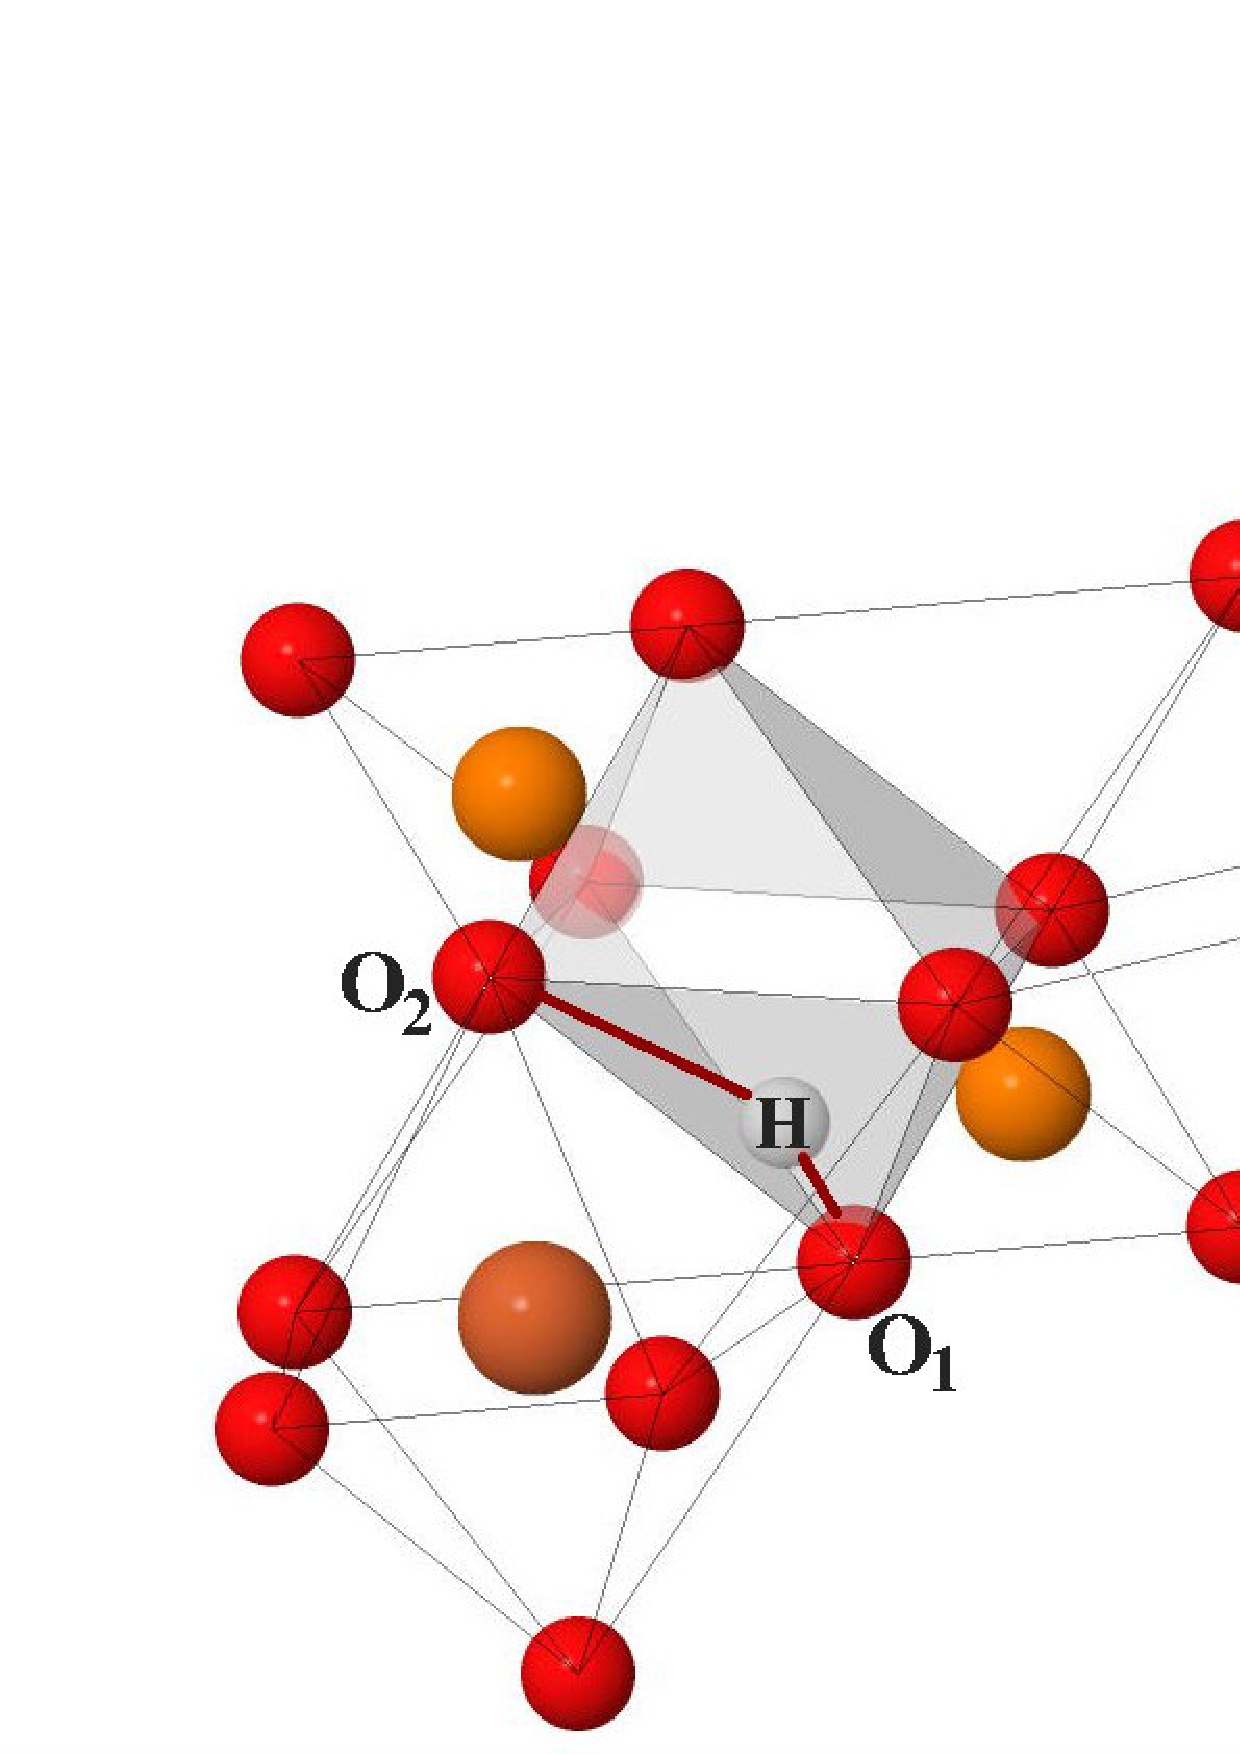
\includegraphics[width=0.9\linewidth]{pictures/oct1beforeCROP.png} \\ a)}
\end{minipage}
\hfill
\begin{minipage}[ht]{0.49\linewidth}
\center{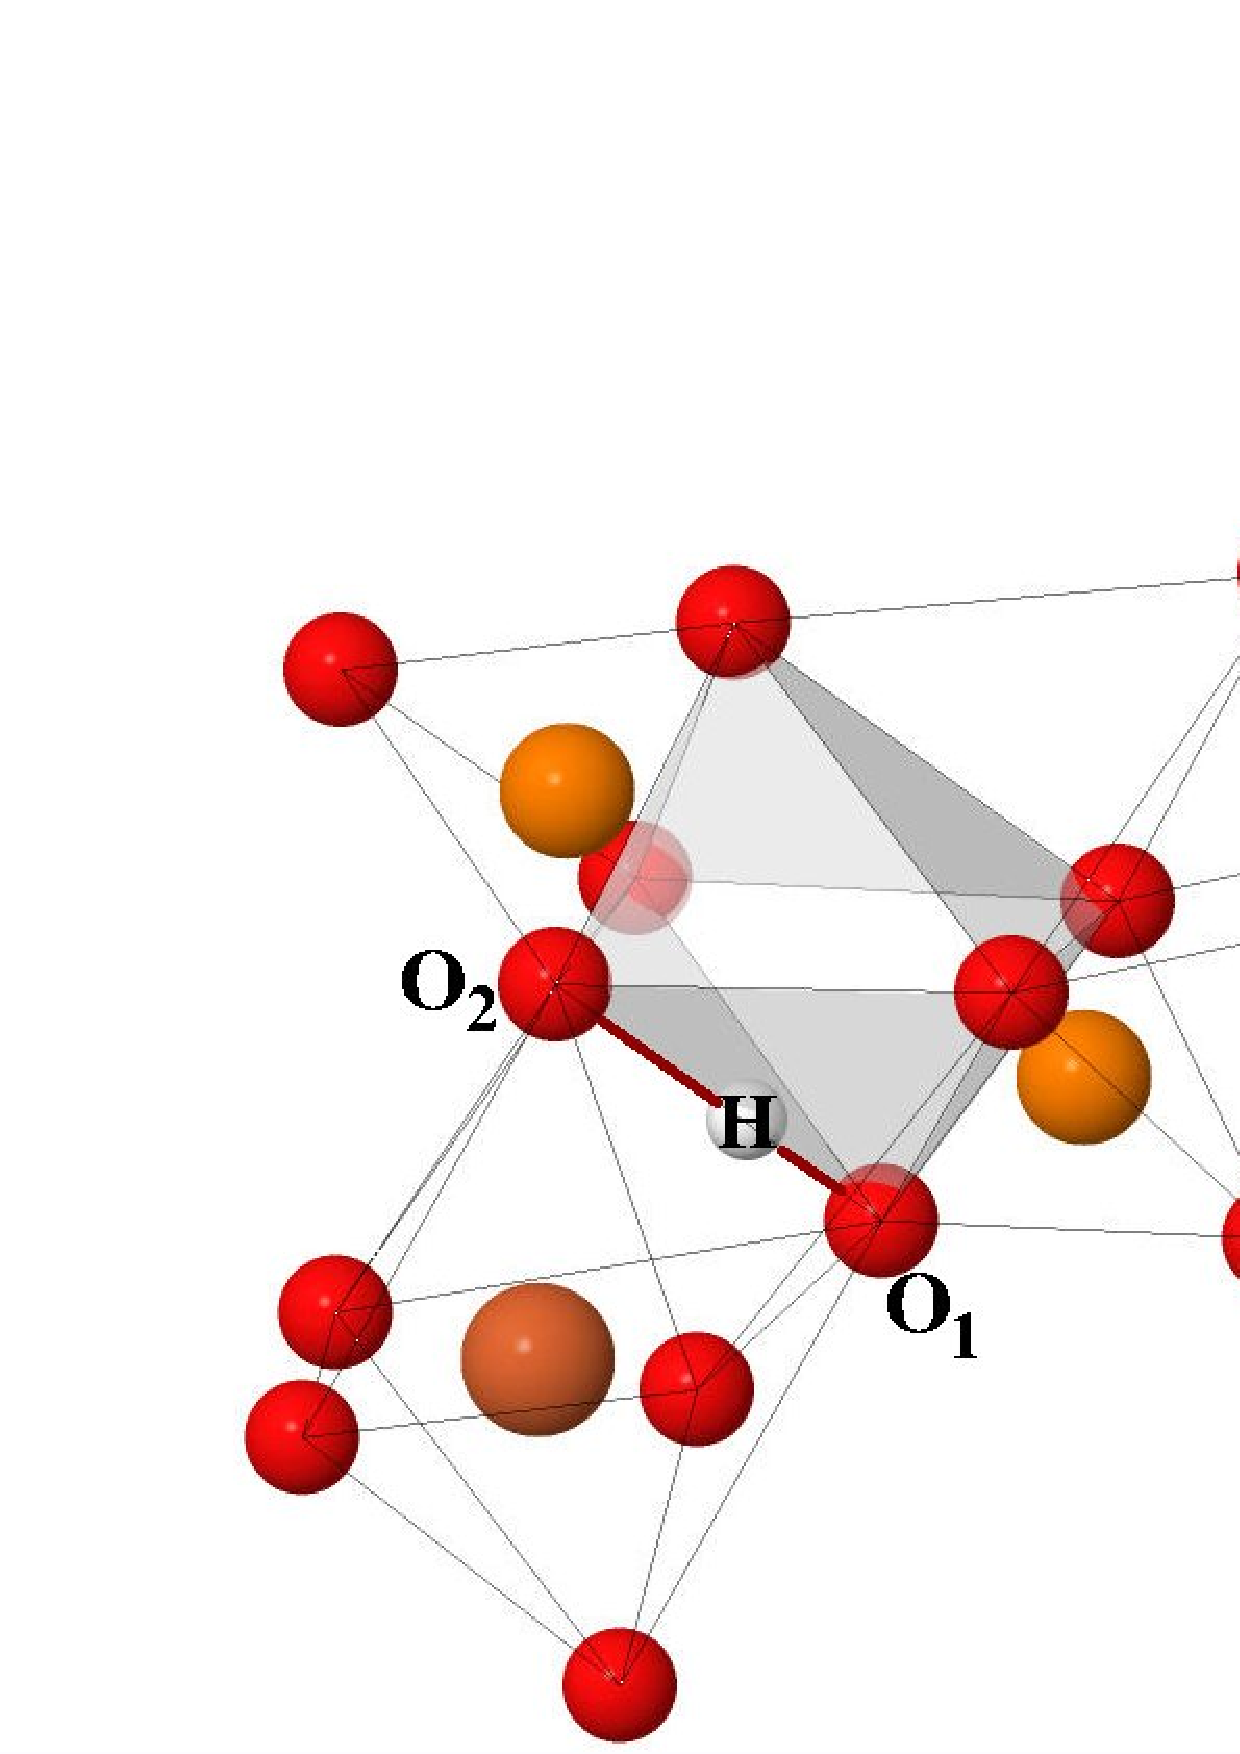
\includegraphics[width=0.9\linewidth]{pictures/oct1afterCROP.png} \\ b)}
\end{minipage}
\caption{Changes of hydrogen localization afret strucrural optimization in 1 case of octahedral void}
\label{ris:oct1}
\end{figure}

\begin{figure}[ht]
\begin{minipage}[h]{0.49\linewidth}
\center{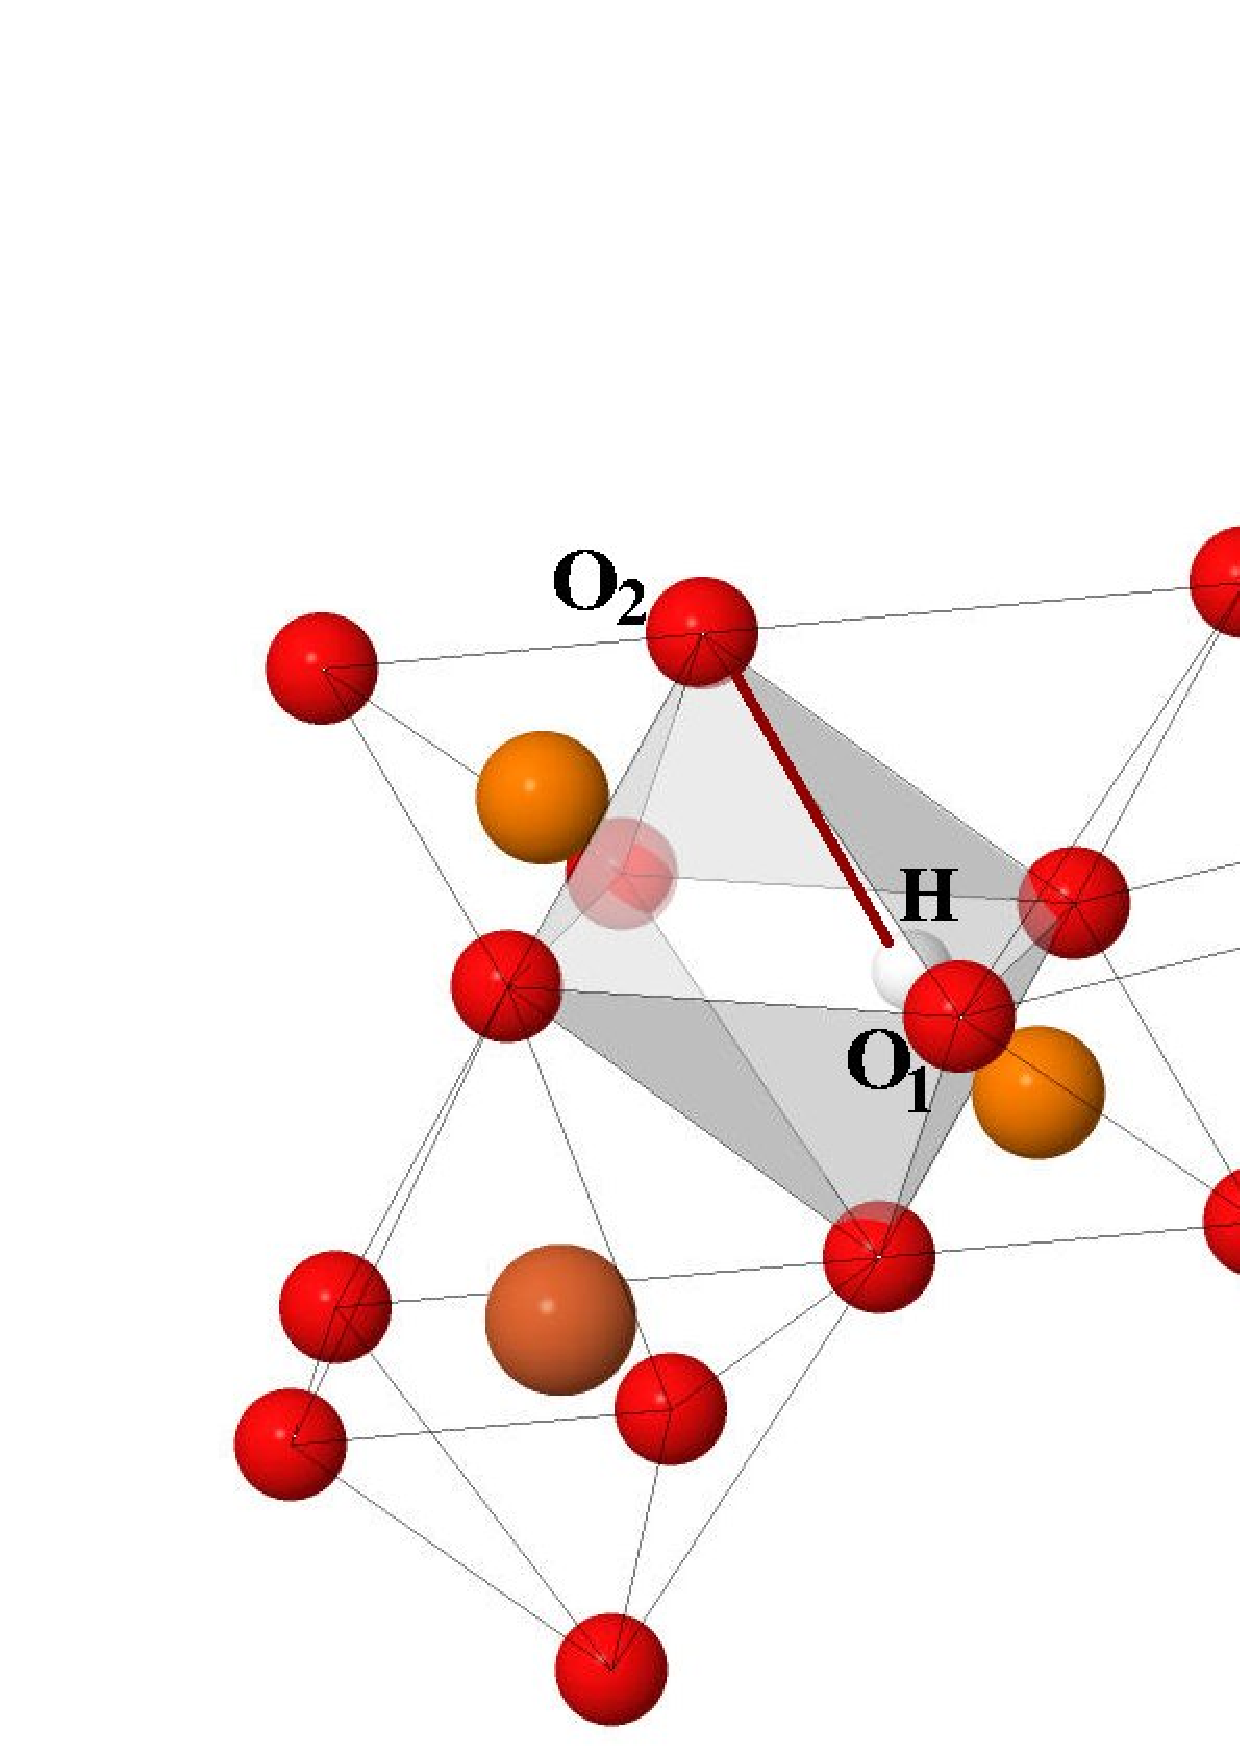
\includegraphics[width=0.9\linewidth]{pictures/oct2beforeCROP.png} \\ a)}
\end{minipage}
\hfill
\begin{minipage}[ht]{0.49\linewidth}
\center{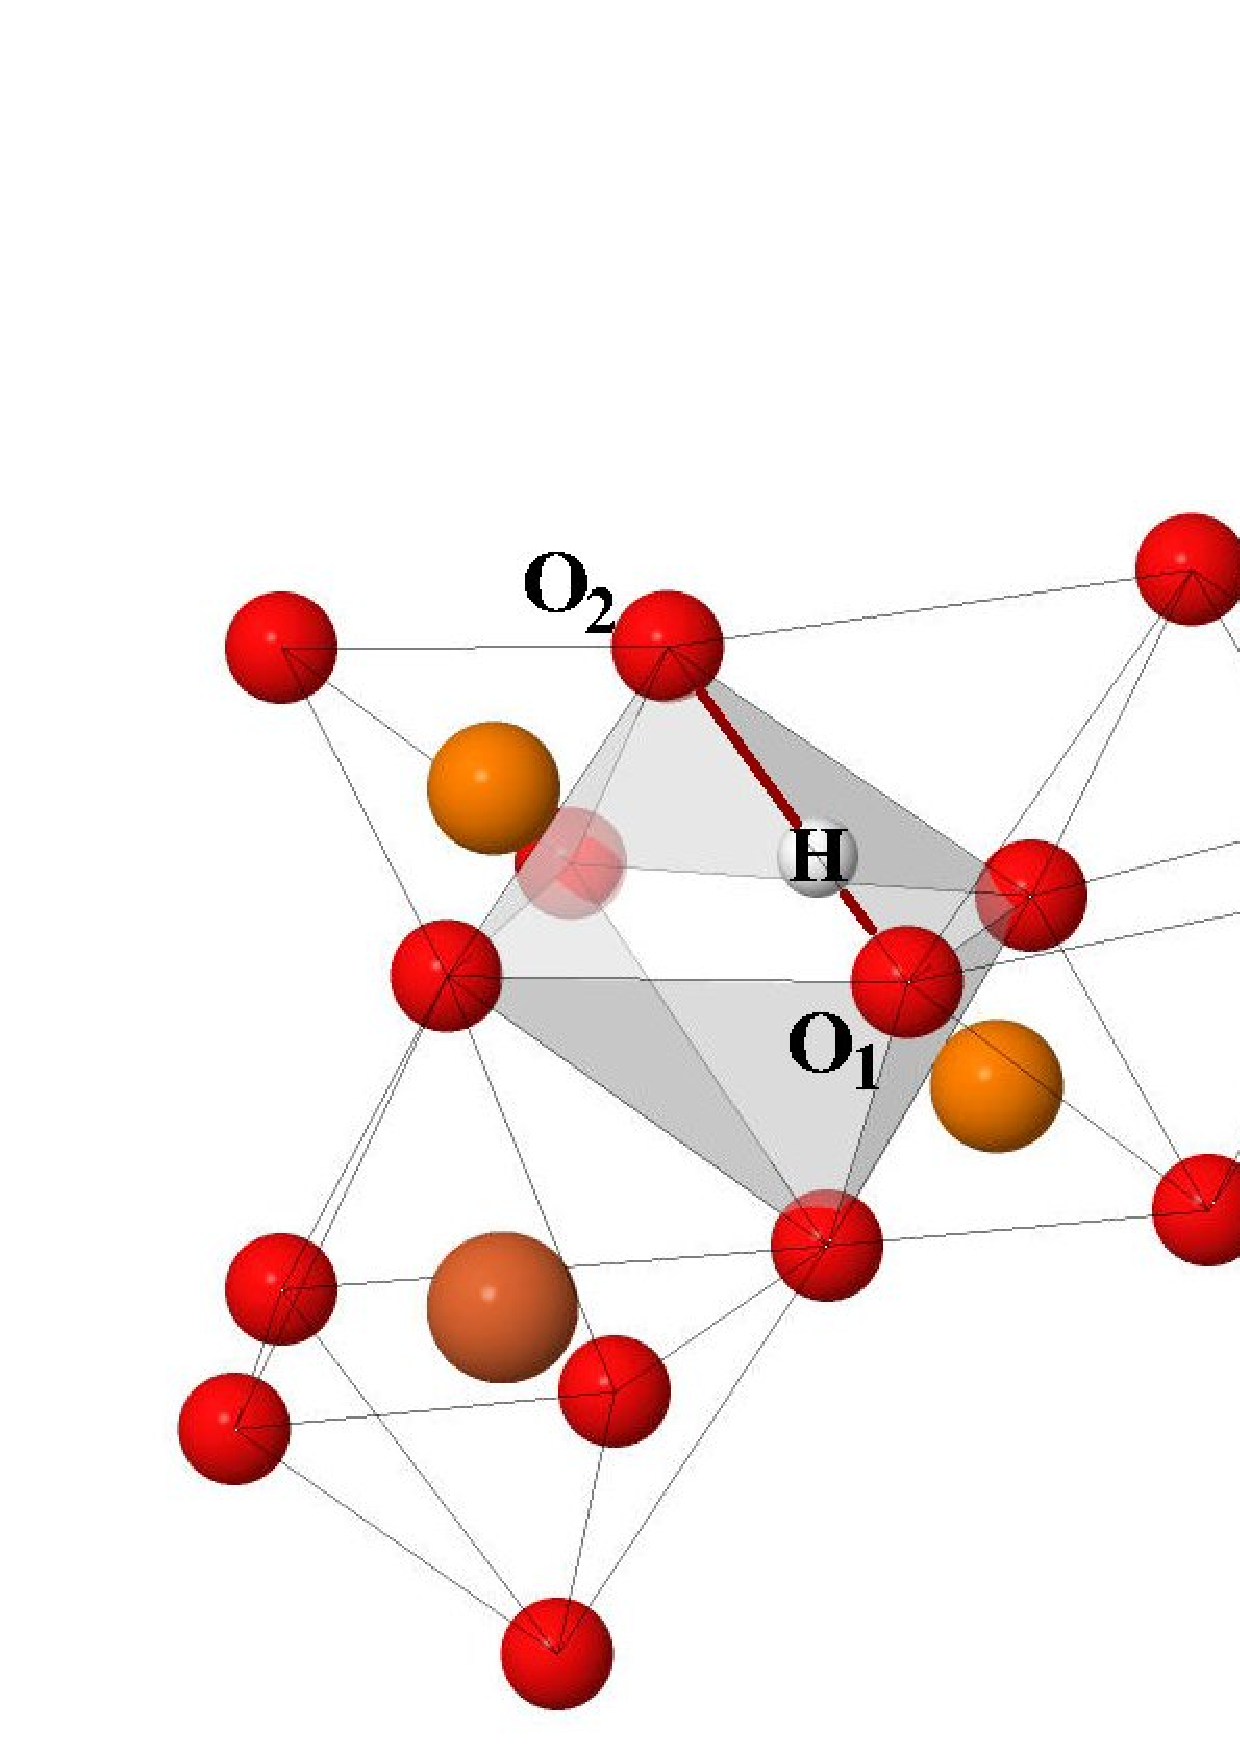
\includegraphics[width=0.9\linewidth]{pictures/oct2afterCROP.png} \\ b)}
\end{minipage}
\caption{Changes of hydrogen localization afret strucrural optimization in 2 case of octahedral void}
\label{ris:oct2}
\end{figure}


\textbf{2. Interstitial hydrogen in tetrahedral void sites of ideeal LFP}

During study of interstitial defects of hydrogen within LFP structure two different configuration of them were found. 
\begin{enumerate}
	\item The first type of hydrogen localization within empty tetrahedral void corresponds to configuration on Fig.\ref{ris:tet1}, where hydrogen locates in the middle of tetrahedral oxygen environment. After relaxation of all positions of atoms, distances between interstitial hydrogen and other atoms are changed: H-O$_1$ from 1.84 \AA to 2.54 \AA; H-O$_2$ from 1.69 \AA to 1.54 \AA; H-Fe from 2.09 \AA to 1.48 \AA. It is important to note the change of distance between O$_2$ atom and neighboring iron: it increases from 2.21 \AA to 2.98 \AA. The formation energy of such defect is equal to -0.7633 eV.
	\item Second interstitial hydrogen defect in tetrahedral void site is located close to iron octahedral site with distance H-O$_1$ is equal to 1.2 \AA, which have changed to 0.99\AA after relaxation of atom positions. Generally, the position of hydrogen changes slightly, Fig.\ref{ris:tet2}. The formation energy of such defect is equal to -0.6676 eV.	
\end{enumerate}


\begin{figure}[ht]
\begin{minipage}[h]{0.49\linewidth}
\center{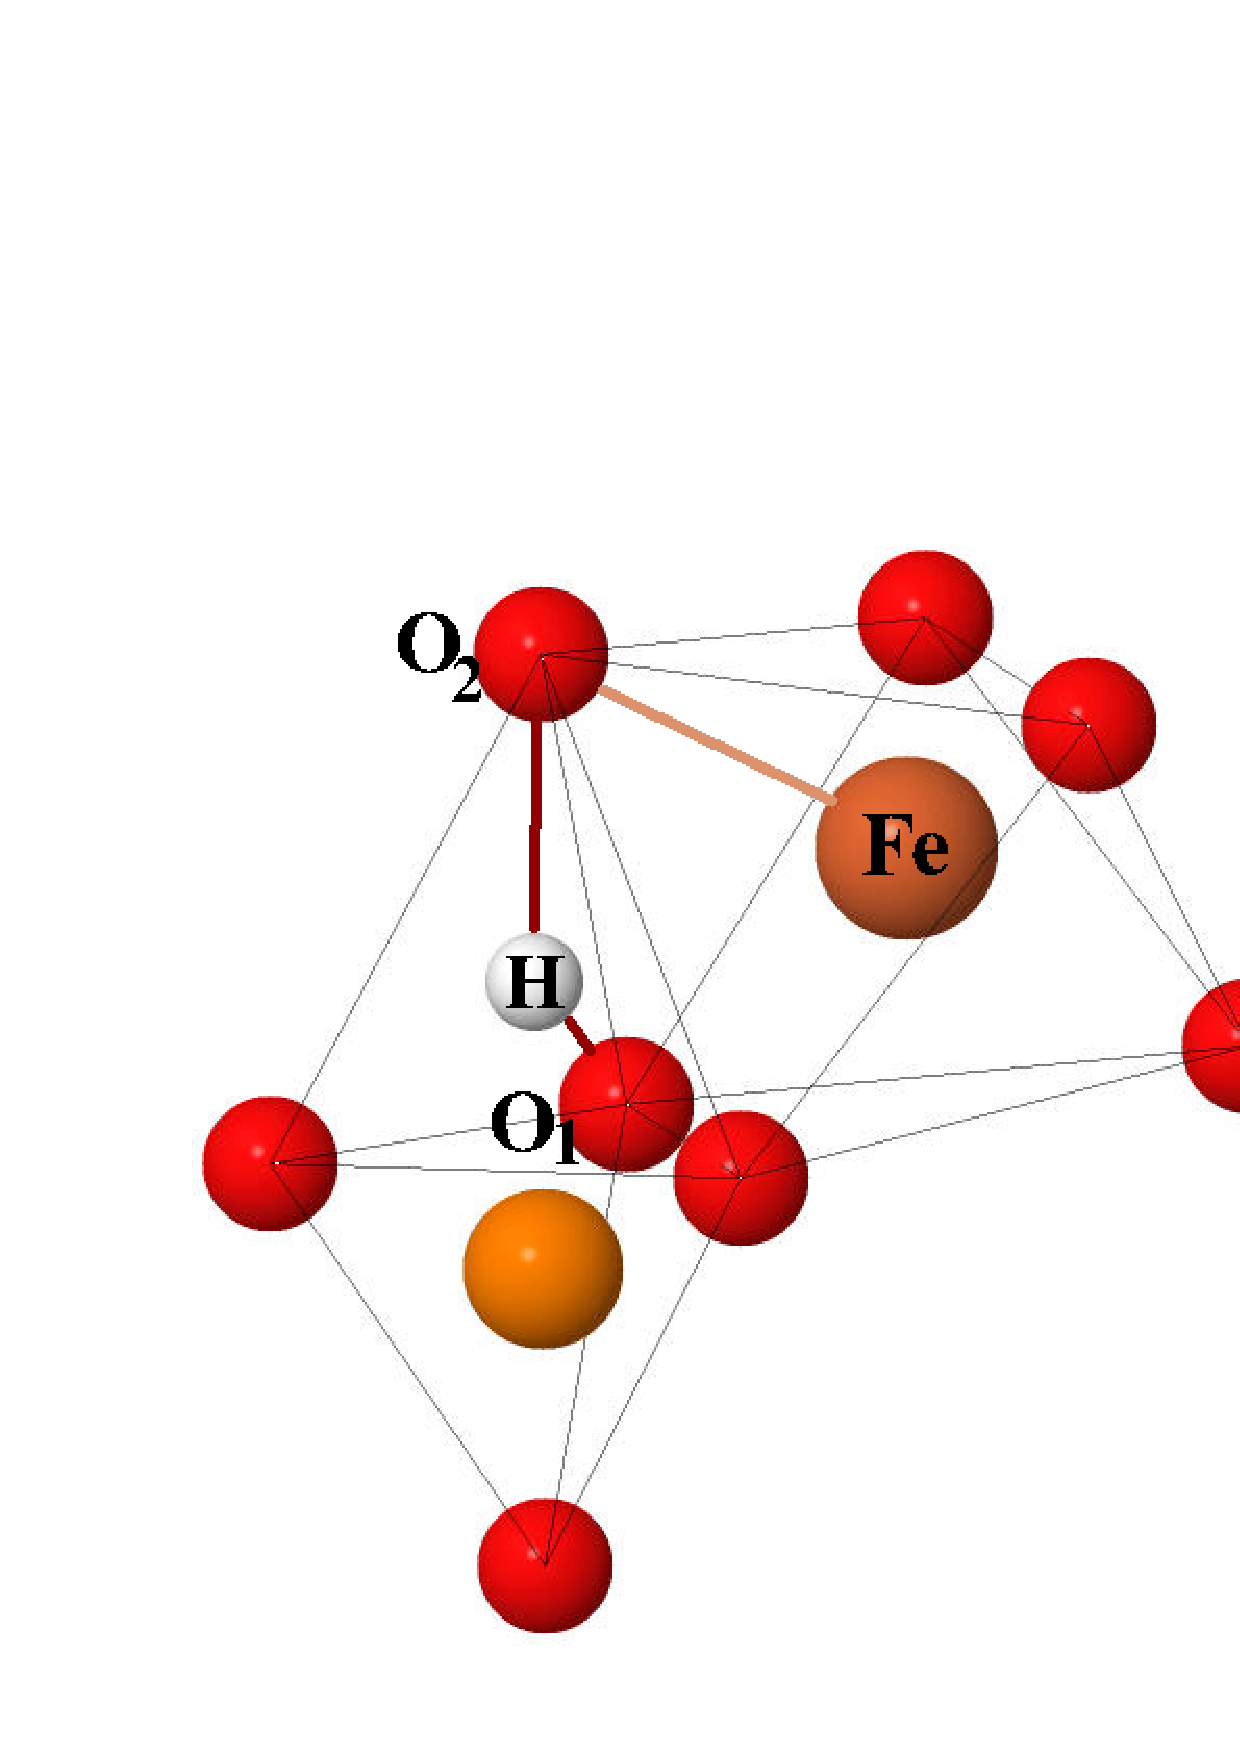
\includegraphics[width=0.9\linewidth]{pictures/tet1beforeCROP.png} \\ a)}
\end{minipage}
\hfill
\begin{minipage}[ht]{0.49\linewidth}
\center{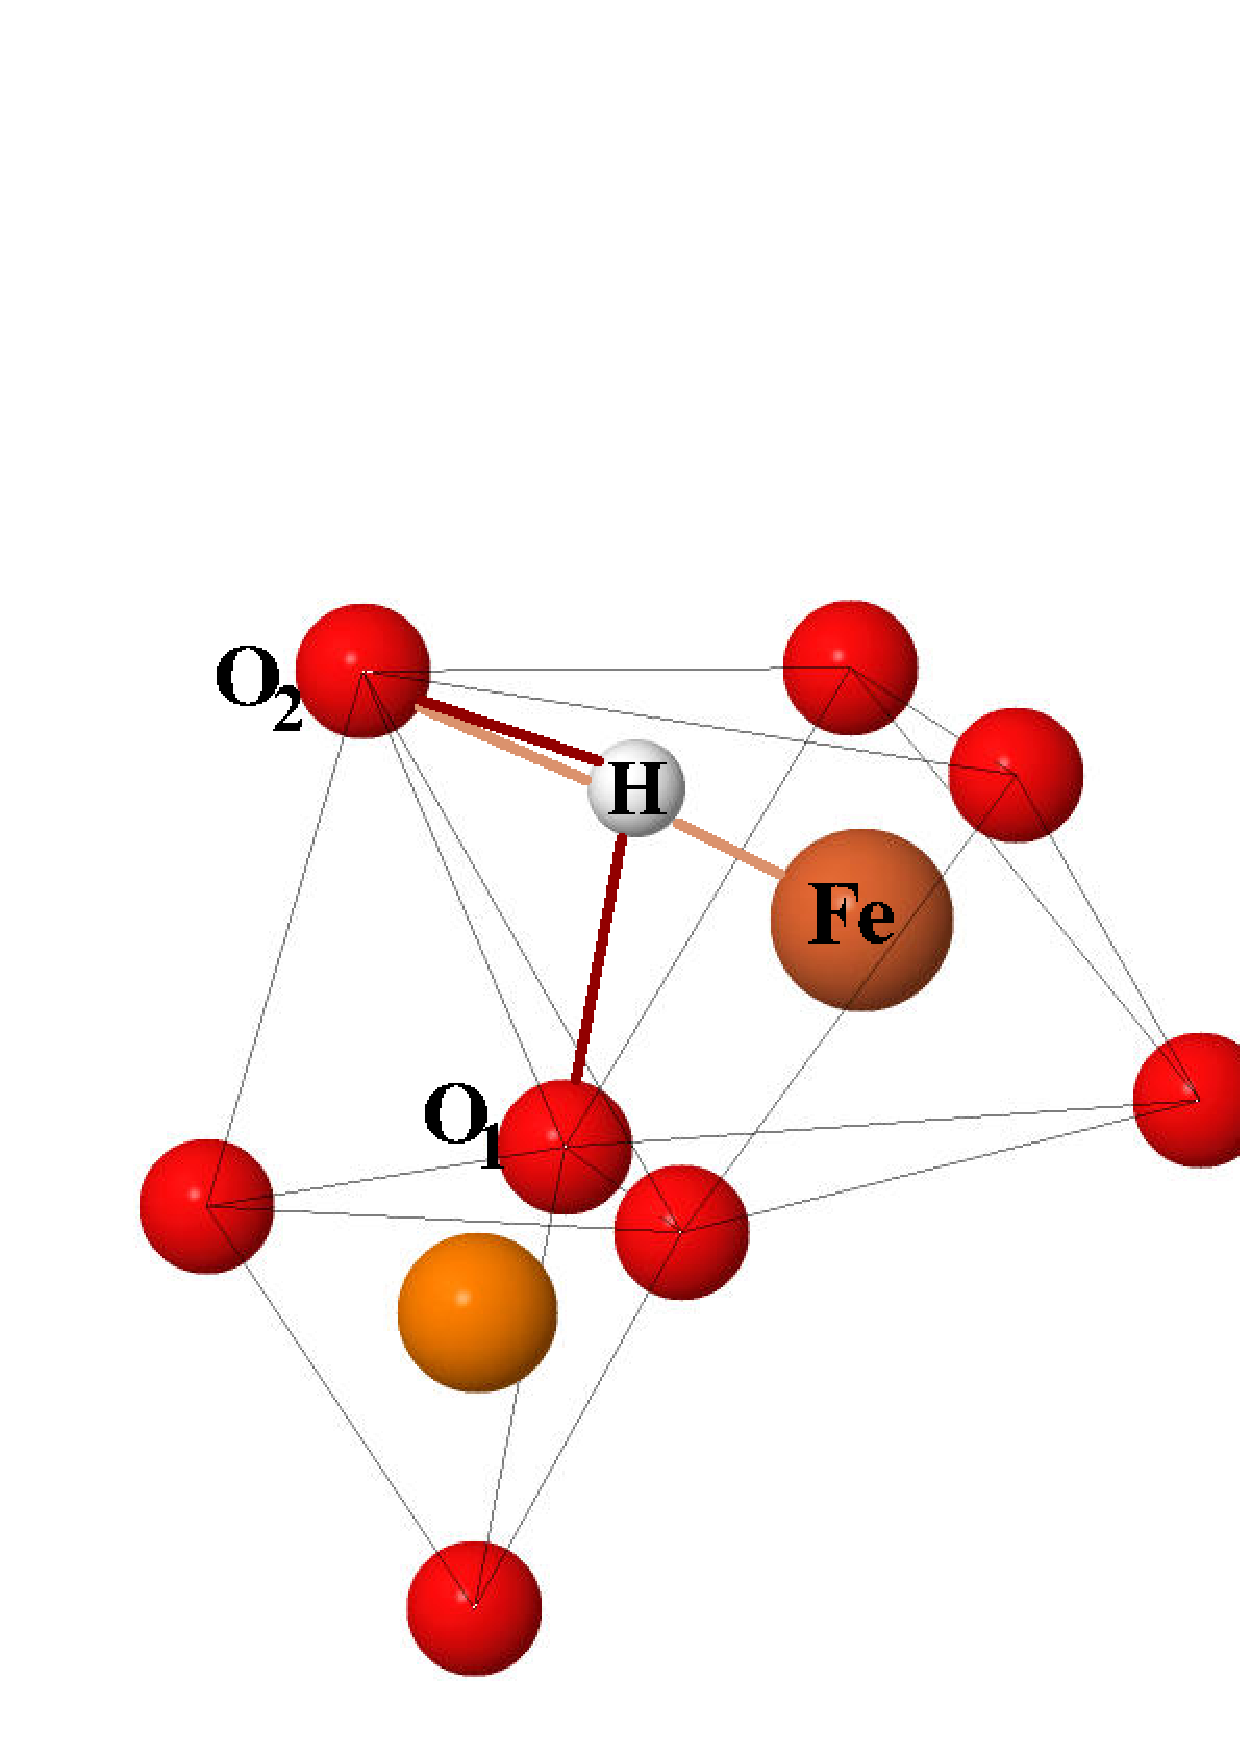
\includegraphics[width=0.9\linewidth]{pictures/tet1afterCROP.png} \\ b)}
\end{minipage}
\caption{Changes of hydrogen localization afret strucrural optimization in 1 case of tetrahedral void}
\label{ris:tet1}
\end{figure}

\begin{figure}[h]
\begin{minipage}[h]{0.49\linewidth}
\center{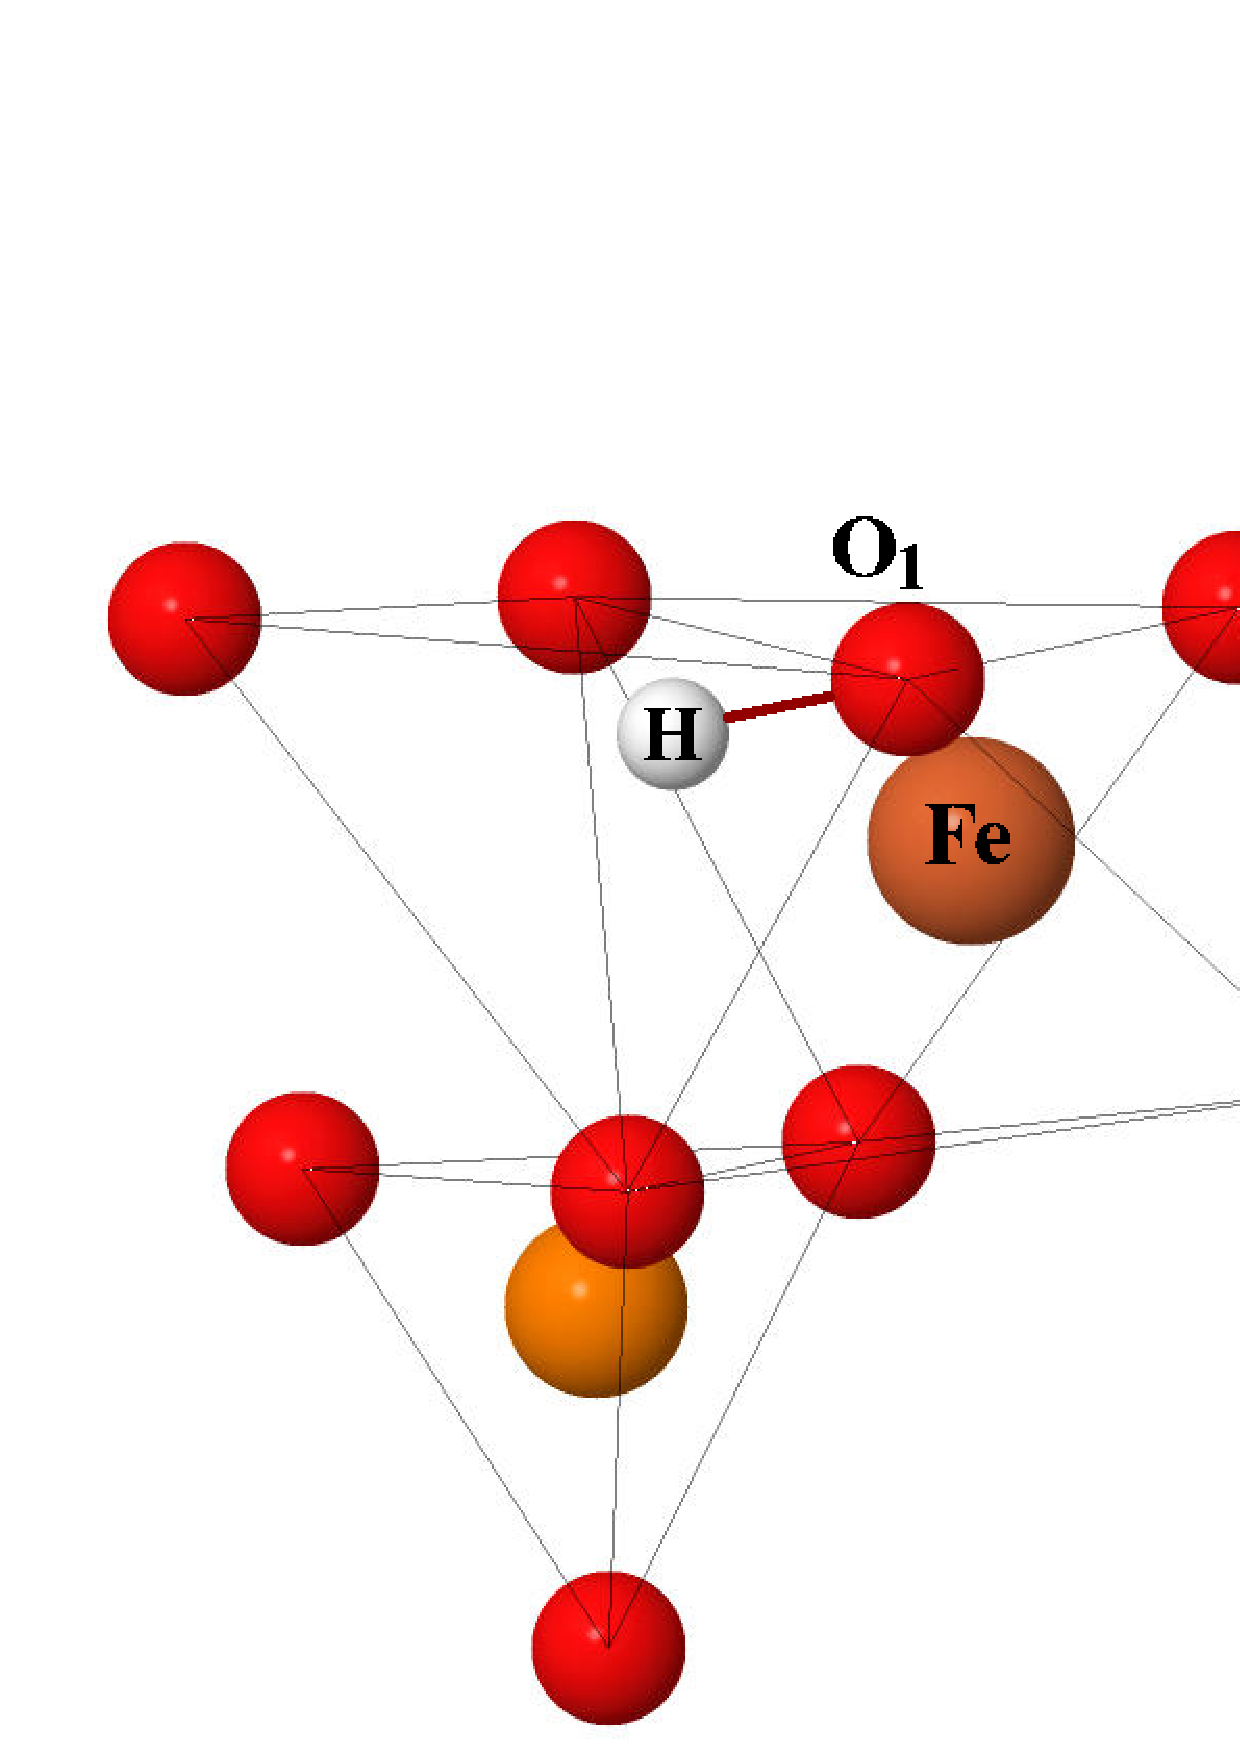
\includegraphics[width=0.9\linewidth]{pictures/tet2beforeCROP.png} \\ a)}
\end{minipage}
\hfill
\begin{minipage}[h]{0.49\linewidth}
\center{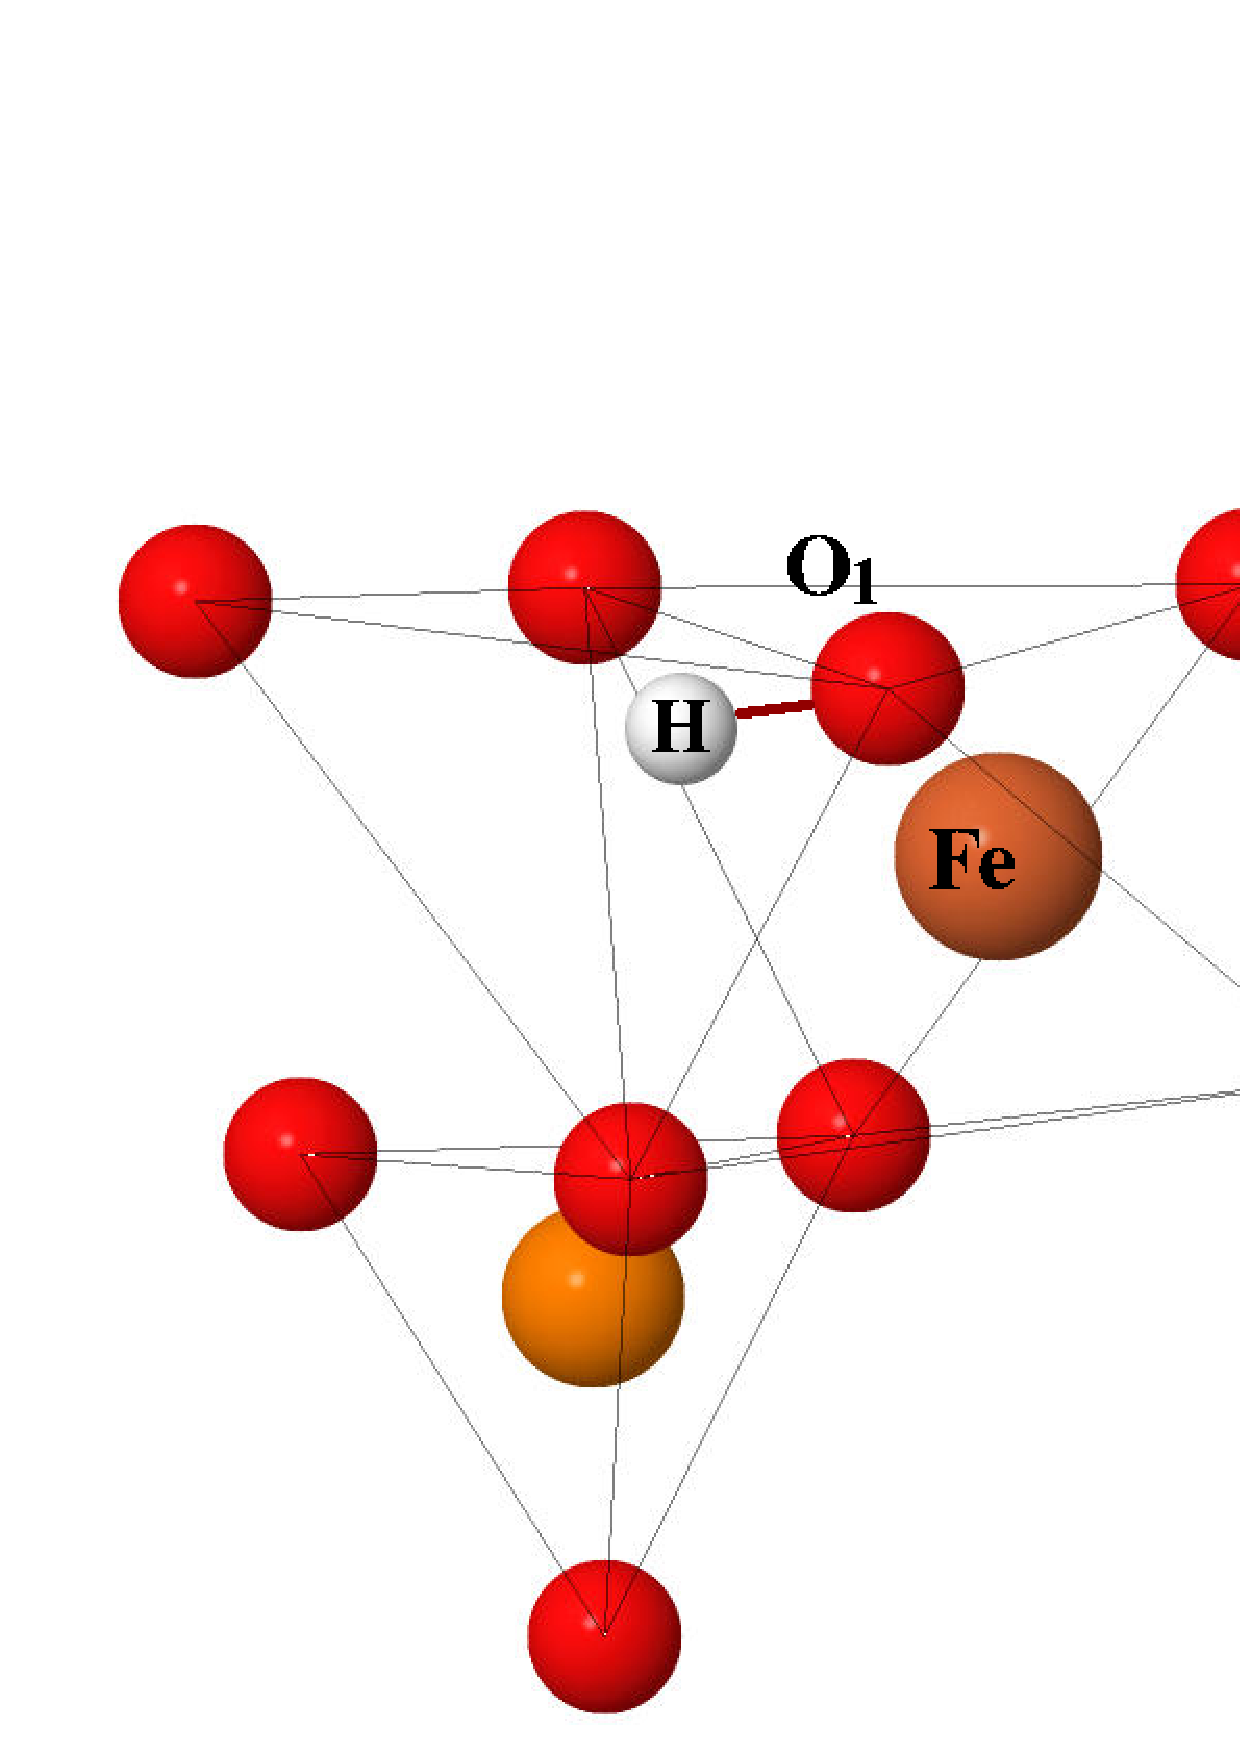
\includegraphics[width=0.9\linewidth]{pictures/tet2afterCROP.png} \\ b)}
\end{minipage}
\caption{Changes of hydrogen localization afret strucrural optimization in 2 case of tetrahedral void}
\label{ris:tet2}
\end{figure}

\textbf{3. Interstitial hydrogen in combination with lithium vacancy in LFP}

For each of possible configurations of interstitial hydrogen within pure LFP the situation with deintercalated lithium was considered. As example, the structure of LFP with interstitial hydrogen in first type of octahedral void site will be discussed below and the table of change in energy for possible configurations will be provided.

For LFP with hydrogen in place of octahedral void site in couple with lithium deintercalated atom the change of its localization are presented in Fig.\ref{ris:oct1-Li}. Distances between heighboring atoms were changed like: Fe-H from 1.99 \AA to 2.04 \AA; H-O$_1$ from 1.99 \AA to 1.02 \AA; H-O$_2$ from 1.55 \AA to 1.67 \AA. Generally, for all possible interstitial position the change of configuration of atoms and relative distanced have really small amount, and the energy of unit cell was changed slightly too. All of these results are provided in Table \ref{tabular:Liinter}.  

\begin{figure}[h]
\begin{minipage}[h]{0.49\linewidth}
\center{\includegraphics[width=0.9\linewidth]{pictures/oct1before-LiCROP.png} \\ a)}
\end{minipage}
\hfill
\begin{minipage}[h]{0.49\linewidth}
\center{\includegraphics[width=0.9\linewidth]{pictures/oct1after-LiCROP.png} \\ b)}
\end{minipage}
\caption{Changes of hydrogen localization after strucrural optimization in 1 case of octahedral void with deintercalated lithium atom}
\label{ris:oct1-Li}
\end{figure}

\clearpage


%\caption{Characteristics of different defects}
\begin{adjustbox}{angle=90}
    %\begin{table}[h!]
    \centering
        %\centering
        \resizebox{18cm}{!}{
        \begin{tabular}{|c|c|c|c|c|c|c|c|}
            %& & & & & &\\
            \hline
            \textbf{Type} & \textbf{Neighborhood} & \textbf{Initial}& \textbf{Relax} & \textbf{Relax+Li$_{vac}$} & \textbf{E$_{form}$ of} & \textbf{E$_{form}$ +U} & \textbf{E$_{form}$ of } \\
            & & & & & \textbf{H$_{defect}$, eV} & & \textbf{H$_{defect}$+Li$_{vac}$, eV} \\
            \hline
            %& & & & & & \\
            Octahedral & H-Fe &  1.95 \AA &  1.99 \AA & 2.04 \AA  & -0.47 &  & -0.94 \\ 
            void 1 & H-O$_1$ & 0.99 \AA & 1.04 \AA & 1.02 \AA & & & \\
             & H-O$_2$ & 2.10 \AA & 1.55 \AA & 1.67 \AA & & & \\
            \hline
            %& & & & & &\\
            Octahedral& P-H & 1.16 \AA & 2.09 \AA & 2.19 \AA & -0.60 & & -0.94 \\
            void 2 & H-O$_1$ &  1.04 \AA & 1.01 \AA & 1.00 \AA & & &\\
            & H-O$_2$ & 2.52 \AA & 1.84 \AA& 2.07 \AA & & &\\
            \hline
            %& & & & & &\\
            Tetrahedral 1 & H-Fe & 2.09 \AA & 1.48 \AA & 1.47 \AA & -0.77 & & -0.7656 \\
            void  & H-O$_1$ & 1.84 \AA & 2.54 \AA & 2.53 \AA & & &\\
            & H-O$_2$ & 1.69 \AA & 1.54 \AA & 1.61 \AA & & & \\
            \hline
            %& & & & & & \\
            Tetrahedral 2 & H-O$_1$ & 1.2 \AA & 0.99 \AA & 1.00 \AA & -0.67 & & -1.10 \\
            %void 2 &  & & & & & & \\
            \hline
            %& & & & & & \\
            Substitutional &  &  &  &  & a) -1.89 eV & a) –0.34 eV & - \\
            hydrogen in place of  & H-O$_1$ & 0.99 \AA & 1.00 \AA & - & b) -3.05 eV & b) 0.89 eV & - \\
            lithium vacancy  &  & & & & & & \\
            \hline
            %& & & & & & & \\
            Substitutional & H$_1$-O$_1$ & 1.25 \AA & 1.00 \AA & - & a) -0.508 & & - \\
            2 hydrogens in place of  & H$_1$-O$_3$ & 2.71 \AA & - & & b) -2.93 eV & b) 0.88 eV & -\\
            iron vacancy  & H$_2$-O$_2$ & 1.20 \AA & 0.99 \AA & - & & &- \\
            & H$_2$-O$_3$ & 2.00 \AA & 1.94 \AA & - & & & -\\
            \hline
            %& & & & & & & \\
            4 hydrogen & (O-H)$_{1}$ &  & 0.97 \AA &  & a) -3.3307 & & - \\ 
            in P vacancy & (O-H)$_{2}$ & & 1.00 \AA& & b) -2.88 eV & b) 0.53 eV & - \\
            site  & (O-H)$_{3}$ & & 1.00 \AA & & & & \\
            & (O-H)$_{4}$ & & 0.98 \AA & & & & \\
            \hline
            %& & & & & & & \\
            5 hydrogen & (O-H)$_{1}$ & &  0.98 \AA &  & a) -2.8486 & & -\\ 
            in P vacancy & (O-H)$_{2}$ & & 1.01 \AA & &b) -2.49 eV &b) 0.73 eV & -\\
            site  & (O-H)$_{3}$ & & 1.01 \AA & & & & \\
            & (O-H)$_{4}$ & & 0.97 \AA & & & & \\
            & (O-H)$_{5}$ & & 1.04 \AA & & & & \\
            \hline
            \label{tabular:Liinter}
        \end{tabular}}
    %\caption{Characteristics of different defects}
    %\end{table}
\end{adjustbox}



\newpage

\textbf{4. Substitutional hydrogen in place of lithium vacancy within LFP}

The possible configuration of substitutional hydrogen in place of lithium vacancy was observed. In this case the change of localization of hydrogen and relative distences are shown in picture below: during relaxation of atomic structure the distance between hydrogen and neighbooring oxygen H-O$_1$ have been changing from 0.99 \AA to 1.00 \AA, Fig.\ref{ris:Li1H}. The corresponding formation energy of such substitutional defect is equal to -1.8864 eV.

\begin{figure}[h]
\begin{minipage}[h]{0.49\linewidth}
\center{\includegraphics[width=0.9\linewidth]{pictures/Li1HbeforeCROP.png} \\ a)}
\end{minipage}
\hfill
\begin{minipage}[h]{0.49\linewidth}
\center{\includegraphics[width=0.9\linewidth]{pictures/Li1HafterCROP.png} \\ b)}
\end{minipage}
\caption{Changes of substitutional hydrogen in place of lithium vacancy after strucrural optimization}
\label{ris:Li1H}
\end{figure}

\textbf{5. Substitutional hydrogen in place of iron vacancy within LFP}

The next substitutional defect is hydrogen in place of iron atom. According to the valency of the last, two of hydrogen can be placed in the structure with one iron atom absence in order to achieve charging neutrality. The distinction in distance between neighbooring atoms is presented in the Fig.\ref{ris:Fe2H}. In this case distances between first hydrogen and oxygen H$_1$-O$_1$ is changes from 1.25 \AA to 1.00 \AA; H$_1$-O$_3$ - frrom 2.71 \AA to 2.00 \AA. Distanses between second hydrogen and neighbooring oxygens are changed like: H$_2$-O$_2$ from 1.20 \AA to 0.99 \AA, H$_2$-O$_3$ from 2.27 \AA to 1.94 \AA. The formation energy of such type of substitutional defect is equal to -0.5079 eV.


\begin{figure}[h]
\begin{minipage}[h]{0.49\linewidth}
\center{\includegraphics[width=0.9\linewidth]{pictures/Fe2HbeforeCROP.png} \\ a)}
\end{minipage}
\hfill
\begin{minipage}[h]{0.49\linewidth}
\center{\includegraphics[width=0.9\linewidth]{pictures/Fe2HafterCROP.png} \\ b)}
\end{minipage}
\caption{Changes of substitutional hydrogen in place of iron atom vacancy after strucrural optimization}
\label{ris:Fe2H}
\end{figure}

\textbf{6. Substitutional hydrogen in place of phosphorus vacancy within LFP}

The last possible substitutional hydrogen defect is its localization in place of phosphorus vacancy site. If one phosphorus atom are removed from its stable position, five of iron atoms in neighboring area are changed their oxidation state from 2+ to 3+. There can be two scenario of substitutional defects: four or five hydrogen atoms in place of phosphorus vacancy. For atoms of hydrogen can build OH bonds with each of oxygen in tetrahedral environment. In this case just one iron atom have changed its oxidation state. According to achieve charging neutrality and taking into accaunt the valency of phosphorus atom within crystal P$^{5+}$ there are need to use 5 atoms of hydrogen. In this case all iron atoms exist in their oxidation state is equal to 2+ without changing. But, according to energy characteristics, the last situation is less likely, Table \ref{tabular:4or5H}. 

Some small changes of atom positions have been happening in the structure during the relaxation calculation. The comparison between two possible substitutional defects are presented in the Fig.\ref{ris:P45H}.For LFP with phosphorus vacancy and four hydrogen atoms as an impuritythe distances between hydrogen and neighboring oxygen are: (O-H)$_{1}$ = 0.97 \AA, (O-H)$_{2}$ = 1.00 \AA, (O-H)$_{3}$ = 1.00 \AA, (O-H)$_{4}$ = 0.98 \AA. In case of five substitutional hydrogen: (O-H)$_{1}$ = 0.98 \AA, (O-H)$_{2}$ = 1.01 \AA, (O-H)$_{3}$ = 1.01 \AA, (O-H)$_{4}$ = 0.97 \AA, (O-H)$_{5}$ = 1.04 \AA.


\begin{figure}[h]
\begin{minipage}[h]{0.49\linewidth}
\center{\includegraphics[width=0.9\linewidth]{pictures/P4HafterCROP.png} \\ a)P vacancy with 4 H}
\end{minipage}
\hfill
\begin{minipage}[h]{0.49\linewidth}
\center{\includegraphics[width=0.9\linewidth]{pictures/P5HafterCROP.png} \\ b) P vacancy with 5 H}
\end{minipage}
\caption{Substitutional hydrogen in place of P atom vacancy after strucrural optimization}
\label{ris:P45H}
\end{figure}



\begin{table}[h]
\caption{Characteristics of P/4H and P/5H defects}
\label{tabular:4or5H}
\begin{center}
\begin{tabular}{|c|c|c|c|}
\hline
& & & \\
\textbf{Type} & \textbf{Bonds} & \textbf{Distance} & \textbf{E$_{form}$, eV} \\
\hline
& & & \\
4 hydrogen & (O-H)$_{1}$ &  0.97 \AA &  -3.3307 \\ 
in P vacancy & (O-H)$_{2}$ & 1.00 \AA & \\
site  & (O-H)$_{3}$ & 1.00 \AA & \\
& (O-H)$_{4}$ & 0.98 \AA &\\
\hline
& & & \\
5 hydrogen & (O-H)$_{1}$ &  0.98 \AA &  -2.8486 \\ 
in P vacancy & (O-H)$_{2}$ & 1.01 \AA & \\
site  & (O-H)$_{3}$ & 1.01 \AA & \\
& (O-H)$_{4}$ & 0.97 \AA & \\
& (O-H)$_{5}$ & 1.04 \AA & \\
\hline
\end{tabular}
\end{center}
\end{table}

1. 4H
2. 5H 

\clearpage

This work is aimed to study the defects in LiFePO$_4$ cathode material. The calculation of structural and electronic properties of LiFePO$_4$ is the first stage of this work. First of all, the space group of crystal is $Pnma$, the Wyckoff position of atoms are presented in Table \ref{tabular:wyckoff}.  As it was described above, structure of LiFePO$_4$ consist of a hexagonal close packing of oxygen with Li and Fe located in half of the octahedral sites and P in 1/8 of tetrahedral sites. The FeO$_6$ disorted octahedra are corner shared and cross linked by the PO$_4$ groups, forming a three-dimentional network with perpendicular tunnels along the [001] direction \cite{morgan}. 

\begin{table}[h]
\caption{$Pnma$ Wyckoff position of atoms}
\label{tabular:wyckoff}
\begin{center}
\begin{tabular}{|c|c|c|}
\hline
& & \\
 \textbf{The Wyckoff parameter} & \textbf{Element}  & \textbf{Coordinates}  \\
\hline
& & \\
8 d & O3 & $\pm$(x, y, z), $\pm$(x, 1/2-y, z), \\ 
  &  &  $\pm$ (x+1/2, 1/2-y, 1/2-z), \\
 &  &  $\pm$(x+1/2, y, 1/2-z)  \\
\hline
& & \\
4 c & Fe, P, O1, O2 & $\pm$($u$+1/2, 1/4, 1/2-$v$), \\
&  &   $\pm$($u$, 1/4, $v$) \\
\hline
& & \\
4 b & - & \\
\hline
& & \\
4 a & Li & (0, 0, 0), (1/2, 0, 1/2), \\
  &  &  (0, 1/2, 0), (1/2, 1/2, 1/2) \\
\hline
\end{tabular}
\end{center}
\end{table}


First step of study is structural optimization of crystal. As it can be seen from Fig.\ref{tabular:str}, for LiFePO$_4$ the cell compression (decrease of cell parameters) is observed. 

\begin{figure}[h]
\begin{minipage}[h]{0.5\linewidth}
\begin{tabular}{ccc}
Parameter & Initial & Optimized \\
a, \AA & 10.45 & 9.88 \\
b, \AA & 6.09 & 5.79 \\
c, \AA & 4.75 & 4.66 \\
$\alpha$=$\beta$=$\gamma$ & 90 & 90 \\
& & \\
\end{tabular}
\end{minipage}
\hfill
\begin{minipage}[h]{0.35\linewidth}
\center{\includegraphics[width=0.7\linewidth]{pictures/out.jpg}}
\end{minipage}
\caption{Structure parameters of LiFePO$_4$ before and after geomentry optimization}
\label{tabular:str}
\end{figure}

The band structure and density of states (DOS) characterization with respect to Fe atom are provided in Fig.\ref{dos}. As it can be seen the maximum of valence band is formed by d-electrons and the minimum of conductive band from s-electrons of Fe. Band gap of LiFePO$_4$ has the value of 3.6eV, which is in good agreement with references \cite{bgap}.

\begin{figure}[h]
\begin{minipage}[h]{1\linewidth}
\center{\includegraphics[width=1\linewidth]{pictures/band.png}}
\end{minipage}
\caption{Band structure and DOS of LiFePO$_4$ in related to Fe}
\label{dos}
\end{figure}

As it can be observed from Table \ref{tabular:wyckoff}, the 4b Wyckoff position of LiFePO$_4$ is not occupied. Thus, for study of intercalation defect in octahedral environment of oxygen atoms, there can be put hydrogen atom to one of this non-occupied position. Also, there can be the H-defect in tetrahedral environment of oxygen. To investigate the hydrogen point defect in different position there was provided structure optimization of 1$\times$2$\times$2 LiFePO$_4$ with intercalation H-atom, Fig.\ref{tabular:def}. During optimization of structure with H-additional atom, there observed some change of atoms positions. In case of octahedral environment of hydrogen atom there are observed the increase of the pore with hydrogen atom volume, the hedrogen in tetrahedral positions tends to leave the tetrahedral environment, Table \ref{tabular:change}.

\begin{figure}[h]
\begin{minipage}[h]{0.3\linewidth}
\center{\includegraphics[width=1\linewidth]{pictures/oct.jpg}}
\end{minipage}
\hfill
\begin{minipage}[h]{0.3\linewidth}
\center{\includegraphics[width=1\linewidth]{pictures/tet1.jpg}}
\end{minipage}
\hfill
\begin{minipage}[h]{0.3\linewidth}
\center{\includegraphics[width=1\linewidth]{pictures/tet22.jpg}}
\end{minipage}
\caption{Octahedral and two types tetrahedral defect position of hydrogen atom}
\label{tabular:def}
\end{figure}

\begin{table}[h]
\footnotesize{
\caption{The change of bond lenghs in defective LiFePO$_4$}
\label{tabular:change}
\begin{center}
\begin{tabular}{|c|c|c|c|}
\hline
& & & \\
 \textbf{ } & \textbf{octahedral (in/opt)}& \textbf{tetrahedral1 (in/opt)}  & \textbf{tetrahedral2 (in/opt)}  \\
\hline
& & & \\
(x, y, z) & (0.0, 0.5, 0.25) / &  (0.89, 0.37, 0.07) /  & (0.1, 0.12, 0.0) /  \\ 
 & (0.0, 0.5, 0.25)  &   (0.82, 0.37, 0.07) & (0.14, 0.12, 0.93) \\ 
\hline
& & & \\
H-O1, \AA & 1.98 / 2.09 &  1.75 / 3.06 & 1.97 / 2.39 \\ 
\hline
& & & \\
H-O2, \AA & 1.98 / 2.09 & 1.94 / 1.58 & 2.06 / 2.82 \\
\hline
& & & \\
H-O3, \AA & 1.85 / 2.06 & 1.45 / 2.44 & 1.97 / 2.39 \\
\hline
& & & \\
H-O4, \AA & 1.85 / 2.06 & 1.45 / 2.44 & 1.35 / 1.05 \\
\hline
& & & \\
H-O5, \AA & 2.12 / 2.20 &  &  \\
\hline
& & & \\
H-O6, \AA & 2.12 / 2.20 & & \\
\hline
& & & \\
H-Fe, \AA &  & 4.27 / 1.48 &  \\
\hline
\end{tabular}
\end{center}
}
\end{table}

In case of formation energy discussion, there can be observed the lowest energy after optimization of H-defect in tetrahedral positions, Fig.\ref{foren}.

\begin{figure}[h]
\begin{minipage}[h]{1\linewidth}
\center{\includegraphics[width=1\linewidth]{pictures/foren.png}}
\end{minipage}
\caption{Formation energy of H-defects in compare with H$_2$ molecule}
\label{foren}
\end{figure}

In case of study of diffusion path between two probably vacancies (tetrahedral 1 and octahedral 5) there tetrahedral site is more favorable due to its minimum of formation energy, Fig.\ref{difpath}. 

\begin{table}[h]
\caption{The diffusion path of H-atom between tetrahedral (1) and octahedral (5) sites in defective LiFePO$_4$}
\label{tabular:difpath}
\begin{center}
\begin{tabular}{|c|c|c|c|}
\hline
& & \\
 \textbf{ } & \textbf{initial}& \textbf{optimized}  \\ 
\hline
& & \\
1 & (0.89, 0.12, 0.43) &  (0.87, 0.12, 0.43) \\ 
\hline
& & \\
2 & (0.90, 0.09, 0.38) & (0.91, 0.09, 0.36) \\
\hline
& & \\
3 & (0.94, 0.06, 0.34) & (0.91, 0.06, 0.29) \\
\hline
& & \\
4 & (0.97, 0.03, 0.29) & (0.99, 0.04, 0.29) \\
\hline
& & \\
5 & (1.0, 0.0, 1.25) &  (0.0, 0.0, 0.25)  \\
\hline
\end{tabular}
\end{center}
\end{table}

\begin{figure}[h]
\begin{minipage}[h]{1\linewidth}
\center{\includegraphics[width=0.8\linewidth]{pictures/difpath.png}}
\end{minipage}
\caption{Energy difference of the diffusion path of H-atom defect between tetrahedral and octahedral vacansies in LiFePO$_4$}
\label{difpath}
\end{figure}

Finally, this work is aimed to study the defects also in P-vacancy position. In such case of defect there can be observed the change of P-atom with 1, 2, 3 or 4 atoms of hydrogen. During this work the study of four atoms of H in P-atomic position was studied in case of three relative positions: four H-atoms inside the tetrahedron oxide invironment, one of H-atom outside the tetrahedron and two H-atoms outside the terahedron, Table \ref{Ppos}. This table describes the case of close placement of hydrogen atoms to oxygen (less than 0.9 \AA). In all of three positions of hydrogen atoms there are observed the bond between two or three hydrogen atoms inside the crystal with H$_2$ or H$_3$ molecules creating, Fig.\ref{h2}, \ref{h3}. Probably, such binding effect of hydrogen atoms is due to the repulsion between hydrogen and oxygen atoms due to a short connection between them and the predominance of repulsive forces.

\begin{table}[h]
\scriptsize{
\caption{Bond lenght between O and H-atoms in pore of P-vacancy of LiFePO$_4$}
\label{Ppos}
\begin{center}
\begin{tabular}{|c|c|c|c|}
\hline
& & & \\
 \textbf{ } & \textbf{H inside (in/out)}& \textbf{one H outside (in/out)} & \textbf{two H outside (in/out)} \\ 
\hline
& & & \\
H-O1, \AA & 0.74/1.62 & 0.74/1.75 & 0.74/1.97\\ 
\hline
& & & \\
H-O2, \AA & 0.74/1.81 & 0.74/1.95 & 0.74/1.75 \\
\hline
& & & \\
H-O3, \AA & 0.78/0.98 & 0.97/0.97  & 0.97/0.97 \\
\hline
& & & \\
H-O4, \AA & 0.84/0.99 & 0.84/0.99 & 0.81/1,78 \\
\hline
& & & \\
GS energy, eV & -786.5 & -787.4 & -784.9 \\
\hline
& & & \\
to note & H$_2$ molecule in the crystal & H$_2$ molecule in the crystal & H$_3$ molecule in the crystal \\
\hline
\end{tabular}
\end{center}
}
\end{table}

\begin{figure}[h]
\begin{minipage}[h]{0.48\linewidth}
\center{\includegraphics[width=0.9\linewidth]{pictures/in2.jpg}}
\end{minipage}
\hfill
\begin{minipage}[h]{0.48\linewidth}
\center{\includegraphics[width=1\linewidth]{pictures/out2.jpg}}
\end{minipage}
\caption{H$_2$ molecule inside of P-vacancy of LiFePO$_4$ before and after optimization}
\label{h2}
\end{figure}

\begin{figure}[h]
\begin{minipage}[h]{0.48\linewidth}
\center{\includegraphics[width=0.9\linewidth]{pictures/in3.jpg}}
\end{minipage}
\hfill
\begin{minipage}[h]{0.48\linewidth}
\center{\includegraphics[width=1\linewidth]{pictures/out3.jpg}}
\end{minipage}
\caption{H$_3$ molecule inside of P-vacancy of LiFePO$_4$ before and after optimization}
\label{h3}
\end{figure}

In case of larger length between oxygen and hydrogen atoms another placement of hydrogen atoms is observed after optimization, Fig. \ref{h21}, \ref{h31}. There the legth of O-H bond is approximately 0.97-1\AA $ $ in all cases of H placement and there are not H$_2$ or H$_3$ molecules inside the crystal. There are not repulsive forces between oxygen and hydrogen atoms. Also Table \ref{Ppos} and \ref{Ppos1} are provided the ground state energies, which is correspond about more stable solution in compound with 0.97-1\AA$ $ length between O and H atoms.

\begin{table}[h]
\scriptsize{
\caption{Bond lenght between O and H-atoms in pore of P-vacancy of LiFePO$_4$}
\label{Ppos1}
\begin{center}
\begin{tabular}{|c|c|c|c|}
\hline
& & & \\
 \textbf{ } & \textbf{H inside (in/out)}& \textbf{one H outside (in/out)} & \textbf{two H outside (in/out)} \\ 
\hline
& & & \\
H-O1, \AA & 0.96/0.97 & 0.96/0.98 & 0.96/0.98 \\ 
\hline
& & & \\
H-O2, \AA & 1.01/0.98 & 1.01/1.00 & 1.01/1.01 \\
\hline
& & & \\
H-O3, \AA & 0.95/0.97 & 1.08/0.98  & 1.08/0.98  \\
\hline
& & & \\
H-O4, \AA & 1.03/0.97 & 1.03/0.98 & 1.00/0.98 \\
\hline
& & & \\
GS energy, eV & -789.8 & -790.3 & -790.3 \\
\hline
\end{tabular}
\end{center}
}
\end{table}

\begin{figure}[h]
\begin{minipage}[h]{0.48\linewidth}
\center{\includegraphics[width=0.85\linewidth]{pictures/in11.jpg}}
\end{minipage}
\hfill
\begin{minipage}[h]{0.48\linewidth}
\center{\includegraphics[width=1\linewidth]{pictures/out11.jpg}}
\end{minipage}
\caption{H-defect inside of tetrahedral P-vacancy of LiFePO$_4$ before and after optimization}
\label{h21}
\end{figure}

\begin{figure}[h]
\begin{minipage}[h]{0.48\linewidth}
\center{\includegraphics[width=1\linewidth]{pictures/in31.jpg}}
\end{minipage}
\hfill
\begin{minipage}[h]{0.48\linewidth}
\center{\includegraphics[width=0.9\linewidth]{pictures/out31.jpg}}
\end{minipage}
\caption{Two H-vacancy  outside of tetrahedral P-vacancy of LiFePO$_4$ before and after optimization}
\label{h31}
\end{figure}

Thus, this work provided three possible locations of hydrogen atoms defects in solid LiFePO$_4$: unoccupied tetrahedral and octahedral position and phosphorus vacancy in crystal. There were studied the possible ground state solutions and energy. But for complete study it is neseccary to investigate all possible positions (with different lengths and angles between internal and external atoms) for find a global minimum of energy.

\newpage

\section{Potential Energy Surface for hydrogen distribution}

During ISP period the studies of LiFePO$_4$ defect structure on three main research direction were performed:

1. Structure stability of four H-atoms in P-vacancy in tetrahedral oxygen environment;

2. Structure stability of two H-atoms in Li-vacancy in octahedral oxygen environment;

3. Hydrogen grid of possible position of four H-atom in P-vacancy tetrahedral polyhedra and study of structural features of material.

\noindent\mbox{\textbf{Four H-atoms in P-vacansy of tetrahedral polyhedra}}

\begin{figure}[h]
\begin{minipage}[h]{0.3\linewidth}
\center{\includegraphics[width=0.85\linewidth]{pictures/1P4H.jpg}} Conf.1 \\
\end{minipage}
\hfill
\begin{minipage}[h]{0.3\linewidth}
\center{\includegraphics[width=0.85\linewidth]{pictures/2P4H.jpg}} Conf.2 \\
\end{minipage}
\hfill
\begin{minipage}[h]{0.3\linewidth}
\center{\includegraphics[width=0.85\linewidth]{pictures/3P4H.jpg}} Conf.3 \\
\end{minipage}
\vfill
\begin{minipage}[h]{0.3\linewidth}
\center{\includegraphics[width=0.85\linewidth]{pictures/4P4H.jpg}} Conf.4 \\
\end{minipage}
\hfill
\begin{minipage}[h]{0.3\linewidth}
\center{\includegraphics[width=0.85\linewidth]{pictures/5P4H.jpg}} Conf.5 \\
\end{minipage}
\hfill
\begin{minipage}[h]{0.3\linewidth}
\center{\includegraphics[width=0.85\linewidth]{pictures/6P4H.jpg}} Conf.6 \\
\end{minipage}
\vfill
\begin{minipage}[h]{0.3\linewidth}
%\center{\includegraphics[width=0.85\linewidth]{7P4H.jpg}} Conf.7 \\
\end{minipage}
\hfill
\begin{minipage}[h]{0.9\linewidth}
\center{\includegraphics[width=0.3\linewidth]{pictures/7P4H.jpg}} Conf.7 \\
\end{minipage}
\caption{Configurations of (4H)$_{P}$ defects}
\label{pvac7}
\end{figure}

There is the article with investigating the defects in similar olivine structure of Mg$_2$SiO$_4$, \cite{mineral}. In this work the possible positions of four H-atoms in tetrahedral polyhedra with phosphorous vacancy was modeling and the stable solution was finding. Repeating similar reasoning in case of LiFePO$_4$ the stable (first) and non-stable (seventh) positions of hydrogen atoms were find, and these results are in good agreement with article,  Table \ref{4H}. But these are preliminary results because the structures need additional stage of optimization due to the presence of excess pressure in the structure. 

\begin{table}[h]
\scriptsize{
\caption{Possible positions of four H-atoms in phosphorus defect polyhedra}
\label{4H}
\begin{center}
\begin{tabular}{|c|c|c|c|}
\hline
& & & \\
 \textbf{Configuration num.} & \textbf{Energy (1 step), eV} &  \textbf{Energy (2 step), eV} &  \textbf{E$_{conf}$-E$_{conf2}$, eV}\\ 
\hline
&  & & \\
1  & -790.31 & -790.36 & 0.2\\ 
\hline
&  & &\\
2  & -789.40 & -790.56 & 0.0\\
\hline
&  & &\\
3 & -790.17 & -790.27 & 0.03\\
\hline
&  & &\\
4 & -789.35 & -790.34 & 0.22\\
\hline
&  & &\\
5 & --788.85 & -790.03 & 0.53\\
\hline
&  & &\\
6 & -790.05 & -790.01 & 0.55\\
\hline
&  & &\\
7 & -789.71 & -789.87 & 0.69\\
\hline
\end{tabular}
\end{center}
}
\end{table}

\noindent\mbox{\textbf{Structure stability of two H-atoms in Li-vacancy in octahedral oxygen environment}}

In case of hexagonal vacancy position (like Fe or Li) there can be observed the change of Li atom by one hydrogen and iron atom by two hydrogen. But in case of Li-vacancy there was some mistake and two hydrogen atoms in pore of lithium atom were modeling. Schematically such structure is presented in fig.\ref{livac}. Such types of defects are needed in more systematically study in the future.

\begin{figure}[h]
\begin{minipage}[h]{1\linewidth}
\center{\includegraphics[width=0.5\linewidth]{pictures/Li_vac.jpg}}
\end{minipage}
\caption{ Two H-atoms in Li-vacancy octahedral polyhedra}
\label{livac}
\end{figure}

\noindent\mbox{\textbf{Grid of possible position of hydrogen atoms in P-vacancy}}

First of all. there is necessary to create the analitical formula of chemical reaction:

\begin{equation}
\frac{1}{4}O_2 + \frac{1}{2}H_2O + 16 Li^{+}Fe^{2+}P^{5+}O^{2-}_4 = Li^{+}_{15}Fe^{2+}_{16}P^{5+}_{16}O^{2-}_{64} + LiOH
\label{firstreaction}
\end{equation}

\begin{equation}
H_2O + Li^{+}_{15}Fe^{2+}_{16}P^{5+}_{16}O^{2-}_{64} + LiOH = H^{+}_{4}Li^{+}_{16}Fe^{2+}_{15}Fe^{3+}_{1}P^{5+}_{15}O^{2-}_{64} + Li_3PO_4 + H_2O
\label{secondreaction}
\end{equation}
There can be observed the formation of Li defect in water and oxygen environment, (\ref{firstreaction}) and P-defect formation with four hydrogen atoms in pore, (\ref{secondreaction}).

In this case there were observed the possible positions of H-atoms in tetrahedral polyhedra with P-vacancy. There are three different positions of oxygen atoms (in depend of environmental atoms) around which there was build the grif of hydrogen, fig. \ref{PH1}-\ref{PH3}. There can be observed two parallen planes along XY-surface with different atoms: in fig.\ref{PH1} iron atom is located in first plane, two lithium atoms are located in second plane; in fig.\ref{PH2} all atoms - two lithium and one iron, are located in first plane, when second plane has only oxygen atoms with empty polyhedral; in fig.\ref{PH3} one iron atom is located in first plane and one iron with one lithium in second plane. Thus, the structure of environment of oxygen atoms is different, but there is one the same property: all oxygen atoms are surrounded by eight tetrahedral polyhedra (in pictures they are marked by gray numbers) and six octahedral polyhedra (marked by black numbers). The tetrahedral without P-atom is noted in fig.\ref{PH1} with 7 grey number, in  fig.\ref{PH2} with 8 grey number and  in fig.\ref{PH3} with 6 grey number. Other seven tetrahedral polyhedra are not occupied by some atoms in the original LiFePO$_4$ structure. Also each oxygen atoms are occupied by six octahedral polyhedra, three of which are occupied by iron or lithium (for example, in fig. \ref{PH1} it is 1, 5 and 6 black numbers) and three are free (in fig. \ref{PH1} it is 2, 3 and 4 black numbers).

The grid of distribution H-atoms represents the 'cloud' of H-atoms in all possible positions around oxygen, there is the condition on the distance between oxygen and hydrogen (more than 0.9\AA and less than 1.3\AA). To study the potential surface of such distribution of H-atoms near the oxygen atoms of phosphorus tetragonal polyhedra we can chose three different ways:

1. full optimization of geometry (but there are too much atoms around several hundred, that requires a lot of resources to calculation);

2. molecular dynamics calculation to find the potential barriers between possible stable positions;

3. non-relaxation solution of hydrogen atoms energies for first step of potential surface investigating.

In this conditions a non-relaxation way as a first step of potential investigating is in the performance. 
   

\begin{figure}[h]
\begin{minipage}[h]{0.5\linewidth}
\center{\includegraphics[width=0.8\linewidth]{pictures/O1_1.jpg}}
\end{minipage}
\hfill
\begin{minipage}[h]{0.5\linewidth}
\center{\includegraphics[width=0.85\linewidth]{pictures/O1_2.jpg}} 
\end{minipage}
\caption{ Polyhedra around O$_1$(-0.046, 0.125, 0.147) }
\label{PH1}
\vfill
\begin{minipage}[h]{0.5\linewidth}
\center{\includegraphics[width=0.85\linewidth]{pictures/O2_1.jpg}} 
\end{minipage}
\hfill
\begin{minipage}[h]{0.5\linewidth}
\center{\includegraphics[width=0.72\linewidth]{pictures/O2_2.jpg}} 
\end{minipage}
\caption{ Polyhedra around O$_2$(0.095, 0.125, 0.370) }
\label{PH2}
\vfill
\begin{minipage}[h]{0.5\linewidth}
\center{\includegraphics[width=0.85\linewidth]{pictures/O3_1.jpg}} 
\end{minipage}
\hfill
\begin{minipage}[h]{0.5\linewidth}
\center{\includegraphics[width=0.85\linewidth]{pictures/O3_2.jpg}} 
\end{minipage}
\caption{ Polyhedra around O$_3$(0.161, 0.224, 0.143) }
\label{PH3}
\end{figure}


\newpage

%\section{Term Early research project}

During 3 term the scaning part of hydrogen distribution in LiFePO$_4$ was realized. There was two step: first of all, non-ralaxation energy study of hydrogen distribution and, secondly, study of energy for atoms into different possible polydedra positions,  fig.\ref{PH1}. Using VASP with NSW parameter equal to 0, that is mean no electronic relaxation steps, there was performed the calculation of energy of each hydrogen atoms in different positions, fig.\ref{PH1c} (this picture is in correspond with  fig.\ref{PH1} with thw same numbers of tetraherrals and octahedrals). At these pictures color is indicator of energy of each hydrogen atom: red color corresponds to higer energy, blue - lower energy. In this term it is possible to see that positions near iron or lithium correspond to higer energy and more advantageous position of hydrogen in tetrahedra with phosphorus vacancy (num.3 grey) and free octahedral (num.4 black).

\begin{figure}[h]
\begin{minipage}[h]{0.5\linewidth}
\center{\includegraphics[width=1\linewidth]{pictures/1_color.jpg}}
\end{minipage}
\hfill
\begin{minipage}[h]{0.5\linewidth}
\center{\includegraphics[width=1\linewidth]{pictures/2_color.jpg}} 
\end{minipage}
\caption{ Polyhedra around O$_1$(-0.046, 0.125, 0.147) }
\label{PH1c}
\end{figure}

 For different polyhedra the full-relaxation energy study of hydrogen atoms were performed (except num.1, 5 and 6 black near the iron and lithium atoms due to theirs hight equilibrium energy). The information about equilibrium energy of hydrogen in different positionin compared to a more stable position (num. 4 initial grey polyhedra) is given in the Table \ref{energy1}. There can be clear seen the advantageous position of hydrogen in defective structure: in case of tetrahedral it is fourth tetrahedral. In this situation hydrogen atom moves to the edge of tetrahedral with number three (between two atoms of oxygen - it is clear seen in fig.\ref{4to3}) and has the lower energy compared with other hydrogen positions. The similar movement but in direction to the face of tetrahedral with number 3 can be observed for hydrogen in 2 and 3 black number octahedral, 3 and 7 grey number tetrahedral. The case of movement from 7 tetrahedral to 3 tetrahedra is provided in fig.\ref{7to3}.  So, these hydrogen atoms have low energy. Hydregen atoms from octahedral with number 4 and tetrahedrals with 1, 2, 5, 6 and 8 numbers have the higer energy. In these cases atoms from from their initial positions move to interfaces with 4 black number of octahedral, Table \ref{energy1}.

\begin{figure}[h]
\begin{minipage}[h]{0.3\linewidth}
\center{\includegraphics[width=1\linewidth]{pictures/4i1.jpg}}
\end{minipage}
\hfill
\begin{minipage}[h]{0.3\linewidth}
\center{\includegraphics[width=1\linewidth]{pictures/4o1.jpg}} 
\end{minipage}
\hfill
\begin{minipage}[h]{0.3\linewidth}
\center{\includegraphics[width=1\linewidth]{pictures/4o2.jpg}} 
\end{minipage}
\caption{Movement of hydrogen atom from 4 grey number of tetrahedral position to 3 number tetrahedral position - more stable position: first picture - before relaxation; second and third - after relaxationin in plane 1}
\label{4to3}
\end{figure}

\begin{figure}[h]
\begin{minipage}[h]{0.5\linewidth}
\center{\includegraphics[width=1\linewidth]{pictures/7i1.jpg}}
\end{minipage}
\hfill
\begin{minipage}[h]{0.5\linewidth}
\center{\includegraphics[width=1\linewidth]{pictures/7o1.jpg}} 
\end{minipage}
\vfill
\begin{minipage}[h]{0.5\linewidth}
\center{\includegraphics[width=1\linewidth]{pictures/7i2.jpg}} 
\end{minipage}
\hfill
\begin{minipage}[h]{0.5\linewidth}
\center{\includegraphics[width=1\linewidth]{pictures/7o2.jpg}} 
\end{minipage}
\caption{Movement of hydrogen atom from 7 grey number of tetrahedral position to 3 number tetrahedral position - one of more stable position: pictures on the left side - before relaxation; pictures in the right side - after relaxation in plane 1, 2 and 3}
\label{7to3}
\end{figure}

\begin{table}[h]
\scriptsize{
\caption{Energy of hydrogen in different polyhedra positions around first oxygen}
\label{energy1}
\begin{center}
\begin{tabular}{|c|c|c|}
\hline
& & \\
 \textbf{Polyhedra} & \textbf{Move to (direction)} & \textbf{E-E$_{3,grey}$, eV}\\ 
\hline
& & \\
 \textbf{tetrahedral}  &  & \\ 
\hline
& & \\
4 & 3 grey & 0.000 \\
\hline
& & \\
3 & 3 grey & 0.002 \\
\hline
& & \\
7 & 3 grey & 0.001 \\
\hline
& & \\
8 & 4 black & 0.419 \\
\hline
& &\\
5 & 4 black & 0.416 \\
\hline
& & \\
6 & 4 black & 0.415 \\
\hline
& &\\
1 & 4 black & 0.483 \\
\hline
& &\\
2 & 4 black & 0.432 \\
\hline
& &\\
\textbf{octahedral} & & \\
\hline
& & \\
2 & 3 grey & 0.003 \\
\hline
& &  \\
3 & 3 grey & 0.002 \\
\hline
& & \\
4 & 4 black & 0.420 \\
\hline
\end{tabular}
\end{center}
}
\end{table}

Thus, using results from Table \ref{energy1} I can provide some conclusions:

1. More stable position of hydrogen in defective LFP structure is observed in the bond between two oxygen of tetrahedral with phosphorus vacancy.

2. The hydrogen atoms in the face of phosphorus defective tetrahedra have lower formation energy.

3. Other positions, which provide advantageous position during first non-ralaxation steps, attempt to move to the face of 4 black number and have related high formation energy.

%\section{Term Early research project}

Next stage of investigating the hydrogen defects in system of LiFePO$_4$ is the study of the hydrogen distribution around second oxygen in phosphorus-defective tetrahedral with presence of hydrogen in relevant position corresponding to first oxygen (from first step of study). In this term the energetical features of hydrogens are noted in fig.\ref{HinO1and2}. There can be clear seen that hydrogen atoms inside the tetrahedral with phosphorus defect (8 grey number in Pane 2) have lower energy in comparison with other outside hydrogens (for example, near iron atom in Plane 1 picture).

\begin{figure}[h]
\begin{minipage}[h]{0.5\linewidth}
\center{\includegraphics[width=1\linewidth]{pictures/2OPlane1CUT4.jpg}}
\end{minipage}
\hfill
\begin{minipage}[h]{0.5\linewidth}
\center{\includegraphics[width=1\linewidth]{pictures/2OPlane2CUT4.jpg}} 
\end{minipage}
\caption{Hydrogen distribution around second oxygen in phosphorus-defective tetraherdal (8 grey number)}
\label{HinO1and2}
\end{figure}

During relaxation of system with two hydrogen atoms (near first oxygen in equlibrium position and second oxygen in various position depends on polyhedra) the energy of second hydrogen was calculated and the table \ref{energy2} was completed. According this information, some conclusions can be performed:

1. Hydrogen atom with movement from 5 black number of octahedral position to 7 grey number of tetrahedral position has the lower energy in comparison with other atoms;

2. The similar low-energy state can be observed for hydrogen atoms in 1, 2, 4 octahedral initial positions and 2, 3, 6, 7, 8 tetrahedral initial positions, which have moved to the edge of 6, 7 and 8 grey numbers of tetrahedral positions during relaxation.

3. The energetically-advantageous position also can be observed in 4 grey number of tetrahedral, where the hydrogen atoms from 1, 4 and 5 grey numbers of tetrahedral have been moved.

\begin{table}[h]
\scriptsize{
\caption{Energy of hydrogen in different polyhedra positions around second oxygen}
\label{energy2}
\begin{center}
\begin{tabular}{|c|c|c|}
\hline
& & \\
 \textbf{Polyhedra} & \textbf{Move to (direction)} & \textbf{E-E$_{5,black}$, eV}\\ 
\hline
& & \\
 \textbf{tetrahedral}  &  & \\ 
\hline
& & \\
8 & b/t 6\&8 grey & 0.0007 \\
\hline
& & \\
7 & 7 grey & 0.0008 \\
\hline
& & \\
6 & b/t 6\&8 grey & 0.0011 \\
\hline
& & \\
3 & 6 grey & 0.0011 \\
\hline
& &\\
2 & 7 grey & 0.0012 \\
\hline
& & \\
4 & 1 grey & 0.7166 \\
\hline
& &\\
1 & 1 grey & 0.7185 \\
\hline
& &\\
5 & 1 grey & 0.7185 \\
\hline
& &\\
\textbf{octahedral} & & \\
\hline
& & \\
\textbf{5} & \textbf{7 grey} & \textbf{0.0000} \\
\hline
& &  \\
4 & 6 grey & 0.0003 \\
\hline
& & \\
1 & 7 grey & 0.0003 \\
\hline
& & \\
2 & 6 grey & 0.0007 \\
\hline
& & \\
6 & b/t 6\&8 grey & 0.0022 \\
\hline
\end{tabular}
\end{center}
}
\end{table}

At the pictures below, fig.\ref{O2Finitialfinal}, the movement of two hydrogen atoms from initial positions to final advantageous positions is presented. 

\begin{figure}[h]
\begin{minipage}[h]{0.5\linewidth}
\center{\includegraphics[width=1\linewidth]{pictures/2O5blackinitial.jpg}}
\end{minipage}
\hfill
\begin{minipage}[h]{0.5\linewidth}
\center{\includegraphics[width=1\linewidth]{pictures/2O5blackfinal.jpg}} 
\end{minipage}
\caption{Two hydrogen atoms in phosphorus-defective tetraherdal}
\label{O2Finitialfinal}
\end{figure}

%\section{Distribution of hydrogen around third oxygen atom}

The study of hydrogen distribution around third oxygen atom in phosphorus-defective LiFePO$_{4}$ structure with presence of two hydrogen near first and second oxygen (from 1 and 2 step of investigation) gives the oppotrunity to create a table \ref{energy3} with energy of each hydrogen which has been moved during relaxation. Before that the non-relaxation step shows the distribution of energetical features, which is presented in fig.\ref{HinO1,2and3}. Using this information there can be the assumption about advantageous position of third hydrogen atom near 2 grey tetrahedral and 5 black octahedral positions. 

\begin{figure}[h]
\begin{minipage}[h]{0.5\linewidth}
\center{\includegraphics[width=1\linewidth]{pictures/3OPlane1.jpg}}
\end{minipage}
\hfill
\begin{minipage}[h]{0.5\linewidth}
\center{\includegraphics[width=1\linewidth]{pictures/3OPlane2.jpg}} 
\end{minipage}
\caption{Hydrogen distribution around third oxygen in phosphorus-defective tetraherdal (2 grey number)}
\label{HinO1,2and3}
\end{figure}

The positions of third hydrogen atoms depending on their initial distribution were found after relaxation. This information is formed the table \ref{energy3}, from which the several conclusions can be formulated:

1. Structure with lower energy is formed with third atom, which is moved from 2 black number of octahedral to the edge between 2 grey tetrahedral with 3 black octahedral position. 

2. Another advantageous position of third hydragen can be observed when hydragen moved from 6 black to 5 black octahedrals.

3. Generally, the more appropriate places of third hydrogen atoms locations is 2 grey tetrahedral and 5 black octahedral positions, that is confirmed by the table after relaxation and non-relaxation information. 

\begin{table}[h]
\scriptsize{
\caption{Energy of hydrogen in different polyhedra positions around second oxygen}
\label{energy3}
\begin{center}
\begin{tabular}{|c|c|c|}
\hline
& & \\
 \textbf{Polyhedra} & \textbf{Move to (direction)} & \textbf{E-E$_{2,black}$, eV}\\ 
\hline
& & \\
 \textbf{tetrahedral}  &  & \\ 
\hline
& & \\
2 & b/t 2grey\&3black & 0.512 \\
\hline
& & \\
4 & 2 grey & 0.512 \\
\hline
& & \\
1 & 1 black & 0.514 \\
\hline
& & \\
6 & b/t 2grey\&3black & 0.512 \\
\hline
& &\\
3 & 3 black & 0.514 \\
\hline
& & \\
8 & 5 black & 0.734 \\
\hline
& &\\
7 & 5 black & 0.740 \\
\hline
& &\\
5 & 5 black & 0.902 \\
\hline
& &\\
\textbf{octahedral} & & \\
\hline
& & \\
\textbf{2} & \textbf{b/t 2grey\&3black} & \textbf{0.000} \\
\hline
& & \\
6 & 5 black & 0.190 \\
\hline
& & \\
1 & b/t 2grey\&4grey & 0.511 \\
\hline
& & \\
3 & b/t 2grey\&3black & 0.514 \\
\hline
& & \\
4 & b/t 2grey\&3black & 0.515 \\
\hline
& & \\
5 & 5 black & 0.738 \\
\hline
\end{tabular}
\end{center}
}
\end{table}

At the pictures below, fig. \ref{O3Finitialfinal}, the movement of third atom between initial and final positions is presented.

\begin{figure}[h]
\begin{minipage}[h]{0.5\linewidth}
\center{\includegraphics[width=1\linewidth]{pictures/3Obefore2black.jpg}}
\end{minipage}
\hfill
\begin{minipage}[h]{0.5\linewidth}
\center{\includegraphics[width=1\linewidth]{pictures/3Oafter2black.jpg}} 
\end{minipage}
\caption{Hydrogen movement to stable position around third oxygen in phosphorus-defective LFP}
\label{O3Finitialfinal}
\end{figure}

%\section{Distribution of hydrogen around fourth oxygen atom}

The last stage of hydrogen subsitution of phosphorus is presented in fig.\ref{HinO1,2,3and4}. 

\begin{figure}[h]
\begin{minipage}[h]{0.5\linewidth}
\center{\includegraphics[width=1\linewidth]{pictures/4OPlane1.jpg}}
\end{minipage}
\hfill
\begin{minipage}[h]{0.5\linewidth}
\center{\includegraphics[width=1\linewidth]{pictures/4OPlane2.jpg}} 
\end{minipage}
\caption{Hydrogen distribution around fourth oxygen in phosphorus-defective tetraherdal (2 grey number)}
\label{HinO1,2,3and4}
\end{figure}

According the information about energy of hydrogen adsorption from table \ref{energy4}, the conclusion about place of appropriate of hydrogen localization can be formulated. There are two octahedral (with 3 and 5 grey numbers), close to which the movement of fourth hydrogen is advantageous. But in case of first octahedral place there is some mistake due to its high energy characteristic after relaxation but advantageous feature after non-relaxation step. 

\begin{table}[h]
\scriptsize{
\caption{Energy of hydrogen in different polyhedra positions around fourth oxygen}
\label{energy4}
\begin{center}
\begin{tabular}{|c|c|c|}
\hline
& & \\
 \textbf{Polyhedra} & \textbf{Move to (direction)} & \textbf{E-E$_{3,black}$, eV}\\ 
\hline
& & \\
 \textbf{tetrahedral}  &  & \\ 
\hline
& & \\
5 & b/t 2grey\&1black & 0.056 \\
\hline
& & \\
4 & b/t 4grey\&2grey & 0.181 \\
\hline
& & \\
8 & b/t 2grey\&1black & 0.181 \\
\hline
& & \\
1 & b/t 4black\&5grey & 0.184 \\
\hline
& &\\
7 & 3 black & 0.307 \\
\hline
& &\\
3 & 3 black & 0.309 \\
\hline
& &\\
2 & b/t 2grey\&1black & 0.921 \\
\hline
& &\\
6 & 1 black & 1.212 \\
\hline
& & \\
\textbf{octahedral} & & \\
\hline
& & \\
\textbf{3} & \textbf{3black} & \textbf{0.000} \\
\hline
& & \\
5 & 5 black & 0.001 \\
\hline
& & \\
4 & 1 black & 0.130 \\
\hline
\end{tabular}
\end{center}
}
\end{table}

Thus, the movement of fourth hydrogen atom is presented in fig.\ref{O4Finitialfinal} with corresponding between last picture of final geometry and required structure of hydrogen localization in LiFePO$_{4}$ with phosphorus defect.

\begin{figure}[h]
\begin{minipage}[h]{0.5\linewidth}
\center{\includegraphics[width=1\linewidth]{pictures/4Obefore.jpg}}
\end{minipage}
\hfill
\begin{minipage}[h]{0.5\linewidth}
\center{\includegraphics[width=1\linewidth]{pictures/4Oafter.jpg}} 
\end{minipage}
\caption{Hydrogen movement to stable position around fourth oxygen in phosphorus-defective LFP}
\label{O4Finitialfinal}
\end{figure}

\newpage

\section{Molecular dynamics investigation}

For verification of previous results about localization of hydrogen atom within phosphorus-defective structure of LiFePO$_{4}$ the molecular dymanics method is used. In this application temperature of thermostat is equal to 700 degree of Celsium is used, according to the article \cite{synthesis}. At that temperature during the sintering after hydrothermal synthesis the pure phase of LiFePO$_{4}$
is observed in an experiment. 

\section{Structure of hydrogen defect within LiFePO$_{4}$}

\newpage

\section{Influence of hydrogen defects to lithium intercalation potential}


%\section{Thermodynamical study of possible defects localization}

The main goal of current research is the study of possible localization of hydrogen defect within material. There can be observed several types of defects: within half of octahedral sites and 7/8 of tetrahedral sites, which are free due to their structure, in site of Li or Fe or P vacancy. Each possible location of this defects were investigated and the energetic characteristics were calculated, Table \ref{thermodyn}.


\begin{table}[h]
\scriptsize{
\caption{Thermodynamic study of different defects}
\label{thermodyn}
\begin{center}
\begin{tabular}{|c|c|}
\hline
& \\
 \textbf{Type of defect} & \textbf{ $\delta$ E, eV} \\ 
\hline
& \\
\textbf{tetrahedral 1}  &  -0.012 \\ 
\hline
& \\
\textbf{tetrahedral 2} &  -0.763 \\
\hline
& \\
\textbf{octahedral} & -0.145 \\
\hline
& \\
\textbf{Li vacancy site} & 0.341 \\
\hline
& \\
\textbf{Fe vacancy site} & -0.465 \\
\hline
& \\
\textbf{P vacancy site} &  \\
\hline
\end{tabular}
\end{center}
}
\end{table}

\section{Electronic properties of LiFePO$_4$ with different concentration of H}

\begin{figure}[h]
\begin{minipage}[h]{1.0\linewidth}
\center{\includegraphics[width=1\linewidth]{pictures/bands0.png}}
\caption{Band structures of LiFePO$_4$ with phosphorus defect}
\label{LFP_Pvac_bs}
\end{minipage}
\end{figure}

\begin{figure}[h]
\begin{minipage}[h]{0.48\linewidth}
\center{\includegraphics[width=1\linewidth]{pictures/bands1.png} \\a)}
\end{minipage}
\hfill
\begin{minipage}[h]{0.48\linewidth}
\center{\includegraphics[width=1\linewidth]{pictures/bands2.png} \\b)} 
\end{minipage}
\vfill
\begin{minipage}[h]{0.48\linewidth}
\center{\includegraphics[width=1\linewidth]{pictures/bands3.png} \\c)} 
\end{minipage}
\hfill
\begin{minipage}[h]{0.48\linewidth}
\center{\includegraphics[width=1\linewidth]{pictures/bands4.png} \\d)} 
\end{minipage}
\caption{Band structures of LiFePO$_4$ with different numbers of substitutional hydrogen a) 1H; b) 2H; c) 3H; d) 4H}
\label{LFP_xH_bs}
\end{figure}